\documentclass[a4paper,12pt,oneside]{book}

% output a PDF/A file
\usepackage[a-1b]{pdfx} 

% Fonts and symbols
\usepackage[utf8]{inputenc} % accepts accented characters
\usepackage[T1]{fontenc} % outputs with fonts of T1 series
\usepackage[english]{babel} % language support
\usepackage{amsmath, amssymb, accents, bm, siunitx}

% define margins
\usepackage[width=130mm,top=35mm,bottom=25mm,headheight=15pt]{geometry}

% graphics and layout packages
\usepackage{graphicx}
\graphicspath{{pictures/}}
\usepackage[dvipsnames]{xcolor}
\usepackage{enumerate}
\usepackage[toc,page]{appendix}
\usepackage{titlesec}
\usepackage{emptypage}
\usepackage{pdfpages}

% modify the caption of the figures
\usepackage{caption}
%\captionsetup[figure]{font=small,labelfont=small}

% packages for tables
\usepackage{booktabs}
\usepackage{tabularx}
\usepackage{multirow, multicol, array, makecell}

% Insert fancy headers, titles and other elements
\usepackage{fancyhdr}
\fancyfoot{}
\fancyhead[RO,LE]{\thepage}
\fancyhead[LO]{\nouppercase{\leftmark}}
\fancyhead[RE]{\nouppercase{\rightmark}}
\fancyhead[RE]{\if@mainmatter Chapter \thechapter\fi}
\renewcommand{\chaptermark}[1]{\markboth{#1}{}}
\pagestyle{fancy}
\usepackage[palatino]{quotchap}

\setcounter{secnumdepth}{3} % do numbering also for subsubsections
% \setcounter{tocdepth}{3} % add subsubsections to Table of Contents

% define your own hypenation if the babel package is not precise
\hyphenation{} 

%---- Links ----
\usepackage{csquotes}
\usepackage{hyperref}
\hypersetup{ % transorm the references into hyperlinks
	colorlinks,
	linkcolor=Blue, % link to figures and equations
	linktoc=page,
	citecolor=OliveGreen, % link to bibliography
}

\graphicspath{ {../img/} }

%---- Document -----
\title{Thesis Title}
\author{Gioele Pozzi}
\date{29-04-2020}


\begin{document}

	% hacking the header
	\pagestyle{fancy}
	\makeatletter
	\renewcommand\chaptermark[1]{%
	  \markboth{\MakeUppercase{%
	    \ifnum \c@secnumdepth >\m@ne
	      \if@mainmatter
	        \@chapapp\ \thechapter. \ %
	      \fi
	    \fi
	    #1}}{}%
	}
	\renewcommand\@mkboth[2]{\markboth{#1}{}}
	\makeatother
	
	%% include frontispieces and chapters
	
\includepdf[pages={1}]{../frontispiece/front-eng.pdf}
	\newpage \thispagestyle{empty} \mbox{}
	
\includepdf[pages={1}]{../frontispiece/front-ita.pdf}

	\newpage \thispagestyle{empty} \mbox{}
	\setcounter{page}{1}
	
	\frontmatter % for roman page numbering
	\chapter{Abstract}
\label{Abstract}
\thispagestyle{empty}

This is the abstract of the thesis. It should be $\approx 500$ words long and it must explain what is the context and the content of the thesis. What is the addressed problem? Briefly summarize the proposed methodology/algorithm along with the main advantages and motivations.
Add a sentence about the achieved results and future works.
	\chapter{Sommario}
\label{Sommario}

\thispagestyle{empty}

\indent Una delle funzioni più attrattive della musica è che questa può trasmettere e comunicare emotioni e modulare l'umore di una persona, come descritto in \cite{feng2003popular}. La musica può provocarci lacrime, consolarci quando siamo tristi, farci innamorare.
\\
La cosa più importante è che gli studi fatti finora sulla musica, affermano che le emozioni sono un criterio importante per la ricerca e l'organizzazione dei brani musicali in playlist. Qui diventa fondamentale l'importanza del campo chiamato \textit{music emotion recognition}.
\\ \indent
Al giorno d'oggi, diventa sempre più importante il fatto di catalogare e organizzare la musica degli utenti, a causa dell'incremento di piattaforme di streaming musicale, le quali danno accesso ad un infinito catalogo di brani.
\\
L'automatizzazione del riconiscimento delle emozioni percepite in musica, permette all'utente di organizzare e ricercare la musica in una visione più incentrata sul contenuto.
\\ \indent
Lo scopo di questa tesi è quello di trovare il link tra emozioni percepite durante l'ascolto di un brano musicale attraverso l'analisi del segnale audio in primis, ma anche con l'utilizzo di segnali psicologici.
\\ \indent
L'utilizzo delle emozioni , in generale, è un compito difficile, a causa della natura intrinseca delle emozioni percepite. Ci sono problemi di affidabilità dei dati empirici e la valutazione del modello di predizione, che d'altra parte non sono dei problemi nei casi ben noti di \textit{face recognition} e \textit{speech recognition}.
	\chapter{Acknowledgements}
\label{Acknowledgements}
\thispagestyle{empty}

\vspace{0.5cm}
This thesis is the result of almost a year of work at the Image and Sound Processing Lab.
First I would thank my supervisor...

\vspace{0.5cm}
Thanks to friends.

\vspace{0.5cm}
Thanks to family.

\vspace{1cm}
\begin{flushright}
\textit{N.S.}
\end{flushright}
	\tableofcontents
	\listoffigures
	\addcontentsline{toc}{chapter}{List of Figures} % this command adds the "List of Figures" page to the table of content as if it was a chapter.
	\listoftables
	\addcontentsline{toc}{chapter}{List of Tables}
		
	\mainmatter % for arabian page numbering
	\input{../chapters/1_introduction.tex} 
	\chapter{Theoretical Background on MIR and MER}
\label{chap:TheoreticalBackgroundMIRMER}
\thispagestyle{plain}

\vspace{0.5cm}

\noindent This chapter introduces the readers to the main basics about Music Information Retrieval and Music Emotion Recognition.

\section{Music Information Retrieval}
Music information retrieval (MIR) is the interdisciplinary science of retrieving information from music. MIR is a small but growing field of research with many real-world applications. Those involved in MIR may have a background in musicology, psychoacoustics, psychology, academic music study, signal processing, informatics, machine learning, optical music recognition, computational intelligence or some combination of these.
\\ \indent
MIR is being used by businesses and academics to categorize, manipulate and even create music.
\\
A few application to MIR can be:
\begin{itemize}
	\item Recommended systems: several already exist, but few are based upon MIR techniques, instead making use of similarity between users or laborious data compilation as in \href{https://www.pandora.com}{Pandora}\footnote{https://www.pandora.com}.
	\item Intelligent and adaptive digital audio effects: aim of design a system that determine the settings of audio effects based on the audio content.
	\item Track separation and instrument recognition: like extracting the original tracks as recorded, which could have more than one instrument played per track. Instrument recognition is about identifying the instruments involved into one track.
	\item Automatic music transcription: process of converting an audio recording into symbolic, such score or a MIDI file.
	\item Automatic categorization: common task of MIR is musical genre categorization and is the usual task for the yearly Music Information Retrieval Evaluation eXchange (MIREX).
\end{itemize}

\section{Music Emotion Recognition}
Music Emotion Recognition (MER) aim to research on modeling humans emotion perception of music \cite{yang2011music}, a research topic that emerges in the face of the explosive growth of digital music.
Automatic MER allows users to retrive and organize their music collections in a fashion that is more content-centric than conventional metadata-based methods.
\\
The main challenge is based on the human perception of emotions, their subjective nature of emotion perception. 
Building such a music emotion recognition system, however, is challenging be- cause of the subjective nature of emotion perception. One needs to deal with issues such as the reliability of ground truth data and the difficulty in evaluating the prediction result, which do not exist in other pattern recognition problems such as face recognition and speech recognition. 
\\
MER methods developed try to address the issues related to the ambiguity and granularity of emotion description, the heavy cognitive load of emotion annotation, subjectivity of emotion perception, and the semantic gap between low-level audio signal and high-level emotion perception.

\subsection{Importance of Music Emotion Recognition}
Music plays an important role in human life, even more in the digital age. Never before has such a large collection of music been created and accessed daily by people. Before with the use of compact audio formats with near CD quality such as MP3 and now on with the various streaming services, have greatly contributed to the tremendous growth of digital music libraries.
\\ \indent
Conventionally, the management of music collections is based on catalog metadata, such as artist name, album name, and song title. As the amount of content continues to explode, this conventional approach may be no longer sufficient. The way that music information is organized and retrieved has to evolve to meet the ever increasing demand for easy and effective information access.
\\ \indent
Music, is a complex acoustic and temporal structure, it is rich in content and expressivity. When an individual engages with music as a composer, performer or listener, a very board range of mental processes is involved, including \textit{representational} and \textit{evaluative}. The representational process includes the perception of meter, rhythm, tonality, harmony, melody, form, and style, whereas the evaluative process includes the perception of preference, aesthetic experience, mood, and emotion. The term evaluative is used because such processes are typically both valences and subjective. Both the representational and the evaluative processes of music listening can be leveraged to enhance music retrieval.
According to a study of \href{https://www.last.fm/home}{Last.fm}\footnote{https://www.last.fm/home}, emotion tagging is the third most frequent type of tags (first is genre and second locale) assigned to music pieces by online users.
\\ Even if emotion-based music retrieval was a new idea, a survey conducted in 2004 from \cite{lee2004survey} showed that about 28.2\% of the participants identified emotion as an important criterion in music seeking and organization.
\\ The table \ref{table:browse_music} represent the responses of 427 subjects to the question \textit{"When you search for music or music information, how likely are you to use the following search/browse options?"} \cite{lee2004survey}.
\begin{table}[h!]
\centering
\begin{tabular}{|l | c|}
\hline
Search/Browse by & Positive rate\\ [0.5ex] 
\hline\hline Singer/Performer 			&		96.2\%	\\ 
\hline	Title of work(s) 					& 		91.6\%	\\ 
\hline	Some words of the lyrics 	& 		74.0\% 	\\
\hline	Music style/genre 				&		62.7\%	\\
\hline	Reccomendations 				&		62.2\%	\\
\hline	Similar artist(s)					&		59.3\%	\\
\hline	Similar music 					&		54.2\%	\\
\hline	Associated usage				&		41.9\% 	\\
\hline	Singing								&		34.8\% 	\\
\hline	Theme(main subject)			&		33.4\% 	\\
\hline	Popularity							&		31.0\% 	\\
\hline	\textbf{Mood/emotional state	}	&		\textbf{28.2\%} 	\\
\hline	Time period						&		23.8\% 	\\
\hline	Occasions to use				&		23.6\% 	\\
\hline	Instrument(s)					&		20.8\% 	\\
\hline	Place/event where heard	&		20.7\% 	\\
\hline	Storyline of music			&		17.9\% 	\\
\hline	Tempo								&		14.2\% 	\\
\hline	Record label						&		11.7\% 	\\
\hline	Publisher							&		6.0\% 	\\
\hline
\end{tabular}
\caption{Responses of 427 subjects to the question \textit{"When you search for music or music information, how likely are you to use the following search/browse options?"}}
\label{table:browse_music}
\end{table}

Into another survey \cite{juslin2004expression}, they present findings from an exploratory questionnaire study featuring 141 music listeners (between 17 and 74 years of age) that offers some novel insights.
\\ 
One of the most exciting but difficult endeavors in research on music is to understand how listeners respond to music. It has often been suggested that a great deal of the attraction of music comes from its “emotional powers”. That is, people tend to value music because it expresses and induces emotions.
The table  \ref{table:motivation_music} tries to resume the motivations to the answer \textit{"Why do we listen to music?"}
\begin{table}[h!]
\centering
\begin{tabular}{|l | c|}
\hline
Motive & Ratio\\ [0.5ex] 
\hline\hline "To express, release and influence emotions"	&	47\%	\\ 
\hline "To relax and settle down"										&	33\%	\\
\hline "For enjoyment, fun, and pleasure"							&	22\%	\\
\hline "As company and background sound"						&	16\%	\\
\hline "Because it makes me feel good"								&	13\%	\\
\hline "Because it's a basic need, I can't live without it"		&	12\%	\\
\hline "Because I like, love music"										&	11\%	\\
\hline "To get energized"													&	9\%	\\
\hline "To evoke memories"												&	4\%	\\ 
\hline
\end{tabular}
\caption{Responses of 141 subjects to the question \textit{"Why do you listen to music?"}}
\label{table:motivation_music}
\end{table}

\indent
Some music companies, like  \href{https://www.allmusic.com/moods}{Allmusic.com}\footnote{https://www.allmusic.com/moods}, gives the possibility to search music by emotion labels. With these, the user can retrive and browse artists or albums by emotion.
\\ \indent
Making computers capable of recognizing the emotion of music also enhances the way humans and computers interact. It is possible to play back music that matches the users mood detected from physiological, prosodic, or facial cues. A cellular phone equipped with automatic music emotion recognition (MER) function can then play a song best suited to the emotional state of the user; a smart space (e.g., restaurant, conference room, residence) can play background music best suited the people inside it.

\subsection{Recognizing the perceived emotion of music}
There is a relationship between music and emotions, that has been the subject of much discussion and research in many different disciplines, like philosophy, musicology, sociology.
\\
In psychological studies, emotion are often divided into three categories:
\begin{itemize}
	\item \textit{Expressed emotion}: the ones the performer tries to communicate with the listener.
	\item \textit{\textbf{Perceived emotion}}: represented by music and perceived by the listener.
	\item \textit{Felt or Evoked emotion}: induced by music and felt by the listener.
\end{itemize}

MER focus on perceived emotions because they are less subjective than felt emotions and are often easier to conceptualize. This because felt emotions depends on personal factors and the situation in which the listener processes the song.
From an engineering point of view, one of the main interests is to develop a computational model of music emotion and to facilitate emotion-based music retrieval and organization. MIR community has made many efforts for automatic recognition of the perceived emotion of music, various implementations will be presented further in chapter \ref{chap:StateOfTheArt}.
\\
A typical approach to MER categorizes emotions into a number of classes and applies Machine Learning (ML) techniques to train a classifies. Usually are extracted some features of music to represent the acoustic property of a music piece. Typically, a subjective test is conducted to collect the ground truth needed for training the computational model of emotion prediction. Subjects are asked to report their emotion perceptions of the music pieces.
\\
To learn the relationship between music features and emotion labels have been applied, such as Support Vector Machines (SVMs), Gaussian Mixture Models (GMMs), Neural Networks (NN) and k-nearest neighbor.
\\
After training, the automatic model can be applied to classify the emotion of an input music piece, for example a schematic diagram of the \textit{categorical approach} to MER can be seen in figure \ref{fig:MER_categorical_approach}.

\begin{figure}[h]
    \centering
    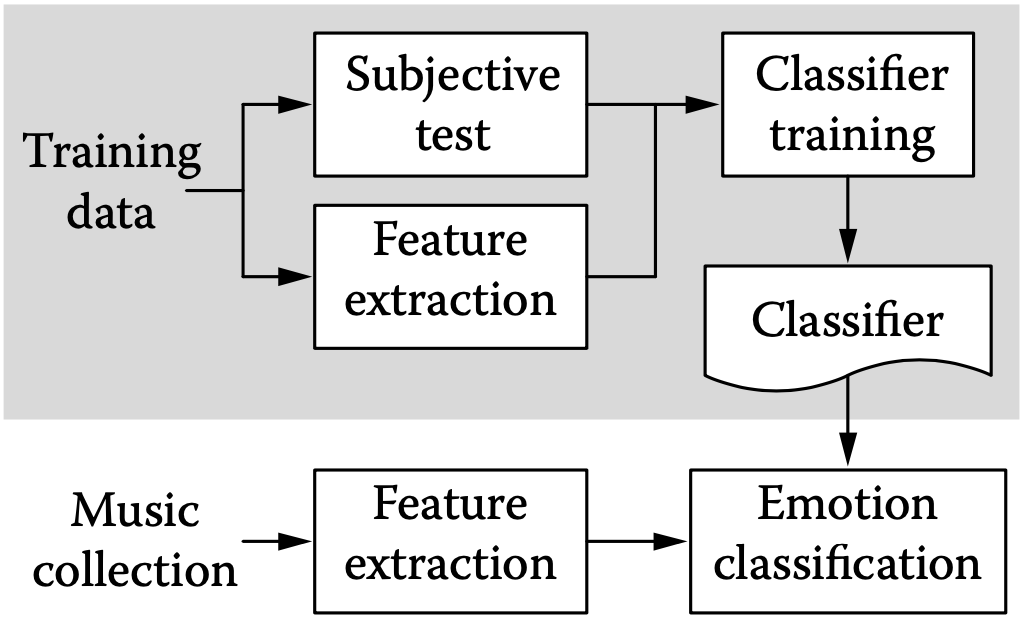
\includegraphics[scale=0.5]{MER_categorical_approach.png} 
	\caption{Schematic diagram of the categorical approach to MER}
    \label{fig:MER_categorical_approach}
\end{figure}

\subsection{Open issues of Music Emotion Recognition} \label{issues}
As MER is a quite new domain, there are some elements that have no clear answer. Four of these issues are:
\begin{enumerate}
	\item Ambiguity and Granularity of emotion description: issue related to the relationship between emotions and the affective terms that denote emotions and the problem of choosing which and how many affective terms to be included in the taxonomy. Emotions are fuzzy concepts, there are main synonyms and similarities between different terms. In general, classification accuracy of an automatic model is inversely proportional to the number of classes considered \cite{van2006emotion}.
	\item Heavy cognitive load of emotion annotation: to collect data for training an automatic model, is typically conducted a subjective test by inviting human subjects to annotate the emotion of music pieces. The problem is that to reduce administrative effort, each music piece is annotated by two or three musical \textit{experts} to gain consensus of the annotation result. Everyday contexts in which musical experts experience is so different from those non-experts require separate treatment. Since MER system is expected to be used in the everyday context, the emotion annotation should be carried out by \textit{ordinary people}.
	\item Subjectivity of emotional perception: music perception is intrinsically subjective and is under the influence of many factors such as cultural background, age, gender, personality and so forth. Therefore conventional categorical approaches that simply assign one emotion class to each music piece in a deterministic manner do not perform very well in practice.
	\item Semantic gap between Low-Level (LL) and audio signal and High Level (HL) Human perception: it is difficult to accurately compute emotion values, and what intrinsic element of music causes a listener to create a specific emotional perception is still far from well understood.
\end{enumerate}

\subsection{Emotion description}
Many researchers have suggested that music is an excellent medium for studying emotion, because people tend to make judgments about music and their affective responses to music.
\\
Music represent emotions that are perceived by the listener or induced emotions that are felt by the listener. Now we will focus on the emotion conceptualization alone, since it's central to have a theoretical background to apply then to MER.
\\
The celebrated paper of Hevner \cite{hevner1935expression} , studied the relationship between music and emotions though experiments where subjects are asked to report some adjectives that came to their mind as the most representative part of a music played. From this have been proposed a large variety of emotion models, like the one presented and used in this thesis.
\\ \indent
The idea of emotion conceptualization is to divide in two different approaches, the \textbf{Categorical approach} and the \textbf{Dimensional approach}.

\paragraph{Categorical approach}
\mbox{} \\ \\ \indent
The first assumption of this emotion conceptualization is that emotions are categorized and categories are distinct from each other. For this approach, there is the idea that there are a limited number of innate and universal emotion categories such as:
\begin{itemize}
	\item Happiness
	\item Sadness
	\item Anger
	\item Fear
	\item Disgust
	\item Surprise
\end{itemize}
All other emotions can be derived from these "\textit{basic emotions}".
\\
In psychological studies, different researchers have come up with different sets of basic emotions.
\\
For example, another famous categorical approach to emotion conceptualization is Hevner's adjective checklist. He found eight clusters positioned in circle as in figure \ref{fig:Hevner_clusters}. The adjective within a cluster are similar, neighbor clusters varies in a cumulative way until reaching the opposite position where there is the contrast cluster. 
\begin{figure}[h]
    \centering
    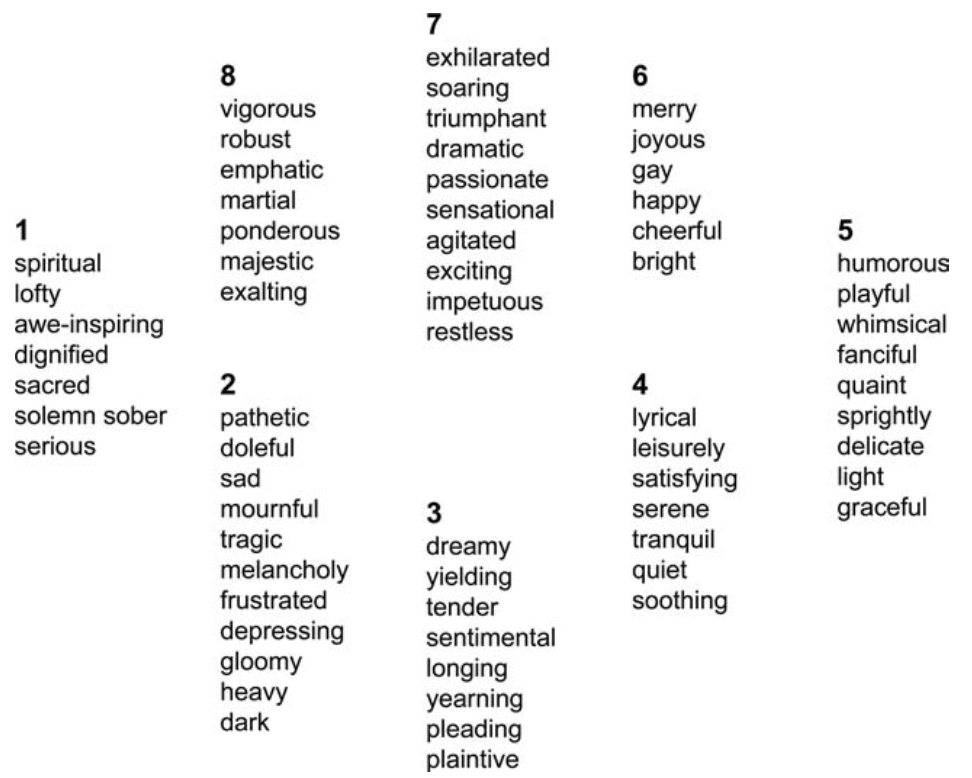
\includegraphics[scale=0.5]{Hevner_clusters.png} 
	\caption{Eight clusters proposed by Hevner}
    \label{fig:Hevner_clusters}
\end{figure}
Hevner's checklist proposed in 1935 was suddenly updated and regrouped into ten groups by Fansworth and into nine groups in 2003 by Schubert.
\\ \indent
Drawbacks of categorical approach is that the number of primary emotion classes is very small in comparison with the richness of music emotion perceived by humans. The problem is in the sense that using a finer granularity, does not necessarily solve the problem because the language for describing emotions is inherently ambiguous and varies from person to person. Using a large number of emotion classes could submerge the subject and is impractical for psychological studies falsing results.

\paragraph{Dimensional approach}
\mbox{} \\ \\ \indent
Categorical approach focuses mainly on the characteristics that distinguish emotions from one another, dimensional approach focuses on identifying emotions based on their position on a small number of emotion "dimensions" called axes, intended to correspond to internal human representation of emotion. These internal emotion dimensions are found by analyzing the correlation between affective terms.
\\ \indent
There are several different names from past researchers gave very similar interpretations of the resulting factors like tension/energy, intensity/softness, tension/relaxation for example. Most of the factors correspond to the two dimensions of emotion the \textit{valence} (positive and negative affective states) and \textit{arousal} (energy and stimulation level).
\\
Russel, proposed a circumplex model of emotion in \cite{russell1980circumplex} which consist in a two-dimensional, circular structure as in figure \ref{fig:Russel_va_model} involving the dimensions of valence and arousal. In this structure, emotions that are inversely correlated, are placed across the circle from one another.
\begin{figure}[h]
    \centering
    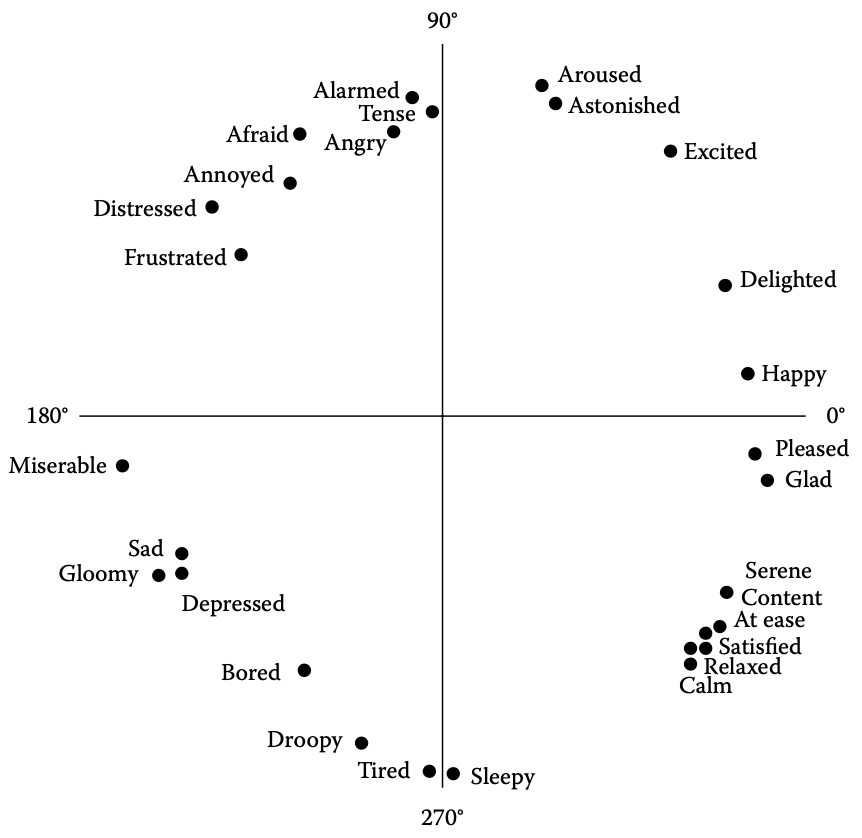
\includegraphics[scale=0.5]{Russel_va_model.png} 
	\caption{Russel's circumplex model of affect}
    \label{fig:Russel_va_model}
\end{figure}

Emotions that are easy to be confused, such as calm and sadness, appear to have similar valence and arousal values. This result implies that valence and arousal may be the most fundamental and most clearly communicated emotion dimensions among others.
Also dimensional approach have its throwbacks, it is argued that dimensional approach blurs important psychological distinctions and consequently obscure important aspects of the emotion process. One example in support of this argumentation is that anger and fear are placed close in the valence-arousal plane but they have very different implications for the organism. Also, it has been argued that using only a few emotion dimension cannot describe all the emotions without residuum.
\\ \indent
Some researches, to overcome to these problems, tries to add a third dimension, called \textit{potency} as dominant/submissive, to obtain a more complete picture of emotion. However, this would increase the cognitive load on the subjects at the same time, requires a more complex interface and makes hard to annotate the process. The third dimension problem is still in discussion.

\paragraph{Music Emotion Variation Detection}
\mbox{} \\ \\ \indent
An important aspect that is not addressed in the previous two paragraphs is the temporal dynamics. Most researches has focused on music piece that are homogeneous with respect to the emotional plane. However, music can change its emotional expression during the song, becomes important to investigate the time-varying relationship between music and emotion. Here is more useful the dimensional approach to capture the continuous changes of emotional expression. Usually subjects are asked to rate valence and arousal in response of the stimulus every second.
\\
For example, songs can be described by valence and arousal curves as in the following figure:
\begin{figure}[h]
    \centering
    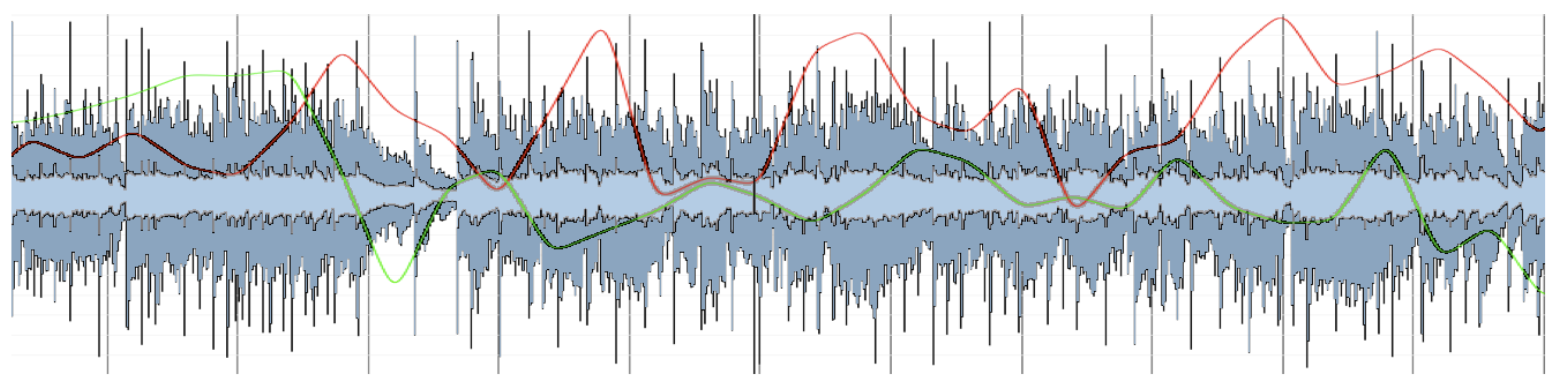
\includegraphics[width=\textwidth]{va_curves.png} 
	\caption{Valence and arousal curves for MEVD}
    \label{fig:va_curves}
\end{figure}

\subsection{Emotion recognition}
MIR researches have been made to automate MER tasks, and the type of music under study has gradually shifted over the past few years from symbolic music to raw audio signal, from Western classical music to popular music. The purpose of MER is to facilitate music retrieval and management in the everyday music listening.
\\ \indent
Nowdays are applied several machine learning techniques to recognize emotion from the music, and the training and automatic recognition model typically consists of the following steps:
\begin{enumerate}
	\item Extract a certain number of features from audio signals to represent the music signal.
	\item Collect from human annotators the ground truth emotion labels or emotion values.
	\item Apply a learning algorithm between music features and emotion labels/values.
	\item Predict emotion of an input song from the resulting computational model.
\end{enumerate}
Researches that work on MER can be classified into three approaches.
\\ \indent
The \textbf{categorical approach} that categorizes emotions into a number of discrete classes and applies machine learning techniques to train a classifier. The predicted emotion labels can be incorporated into a text-based or metadata-based music retrieval system.
\\ \indent
The \textbf{dimensional approach} to MER defines emotions as numerical values over a number of emotion dimensions (valence and arousal). A regression model is trained to predict the emotion values that represent the affective content of a song, thereby representing the song as a point in an emotion space. Users can then organize, browse, and retrieve music pieces in the emotion space, which provides a simple means for user interface.

\paragraph{Categorical approach}
\mbox{} \\ \\ \indent
Advantage of categorical approach is that it is easy to be incorporated into a text-based or metadata-based retrieval system. Emotion labels provide an atomic description of music that allows users to retrieve music through a few keywords. Here are present the issues discussed in chapter \ref{issues}.
The commonly adopted methods follows these points:
\begin{enumerate}
	\item Data collection: nowadays there are several large-scale dataset covering all sort of music types and genres. Otherwise is desirable to collect data of the different types, getting rid of the effects called "\textit{album effect}" or "\textit{artist effect}" and collect a variety of music pieces. One problem is that there is no consensus on which emotion model or how many emotion categories should be used. Comparing systems that use different emotion categories  and different dataset is impossible. However the issue concerning how many and which emotion classes should be used seem to remain open.
	\item Data preprocessing: to compare music pieces fairly, music pieces are normally converted to a standard format, and since a complete music piece can contain sections with different emotions,a 20 to 30 second segment is often selected, which is representative of the song (like the chorus part). A good remark of the segment length can be found in \cite{macdorman2007automatic}.
	\item Subjective test: emotion is a subjective matter, so the collection of the ground truth data should be conducted carefully. Annotation methods can be grouped into two categories:
	\begin{itemize}
		\item Expert-based method: which employs a few musical experts to annotate emotions.
		\item Subject-based method: employs a large number of untrained subjects to annotate emotions.
	\end{itemize}
	The ground truth is set by averaging the opinion of all subjects (typically more than 10 subjects per song).
	\\
	It became important to not make a long test, in order to not compromise the reliability of the emotion annotations. Nowadays is introduced the use of listening games.
	\item Features extraction: a certain number of features are extracted from the music signal to represent the different dimension of music listening like melody, timbre and rhythm.
	\\ After features extraction, is applied feature normalization, in order to 
	\item Model training: the following step is to train a Machine Learning (ML) model to learn the relationship between emotion and music. Music emotion classification is carried out with classification ML algorithms, such as Neural Network, k-nearest neighbor (kNN), decision tree, Support Vector Machine (SVM) and Support Vector Classification (SVC).
\end{enumerate}

\paragraph{Dimensional approach}
\mbox{} \\ \\ \indent
The attractive part of dimensional approach is the valence-arousal plane and the associated emotion-based retrieval methods. Due to the fact that the emotion plane contain an infinite number of emotion descriptions, the granularity and ambiguity issues are relieved.
\\
Dimensional perspective is adopted to track the emotion variation of a classical song. The idea of representing the overall emotion of a popular song as a point in the emotion plane for music retrieval, under the assumption that the dominant emotion of a popular song undergoes less changes than a classical song. MER problem became a regression problem, and two independent models, called regressors, are trained to predict the valence-arousal values.
\\
The dimensional approach requires the subjects to annotate the numerical valence-arousal values. This requirement impose an high cognitive load on the subjects.
\\ \\
Pros and cons of categorical and dimensional approach are schematized in the following table:
\begin{table}[h!]
	\centering
	\begin{tabular}{|c|p{0.35\textwidth}|p{0.35\textwidth}|}
	\hline
	& Pros & Cons\\ [0.5ex] 
	\hline\hline Categorical & Intuitive \newline Natural language \newline Atomic description & Lack a unifying model \newline Ambiguous \newline Subjective \newline Difficult to offer fine-grained differentiation \\
	\hline Dimensional & Focus on a few dimensions \newline Good user interface & Less intuitive \newline Semantic loss in projection \newline Difficult to obtain ground truth \\
	\hline
	\end{tabular}
	\caption{Pros and cons of categorical and dimensional approaches}
	\label{table:pros_cons_categorical_dimensional}
\end{table}

\subsection{Valence and Arousal}
As already mentioned before, the valence-arousal plane is the most used dimension plane to represent emotion.
\\
In general, emotional experiences can be described by these two terms, \textit{valence} (positive or negative affectivity) and \textit{arousal} (calming or exciting). Some studies found that valence as well as intensity, is triggered by the amygdala, while the arousal by the reptilian brain.
\\
The common framework for dealing with emotional experience is characterized in a two-dimensional space. Valence ranges from highly negative to highly positive, and arousal ranges from calming/soothing to exciting/agitating:
\begin{figure}[h]
    \centering
    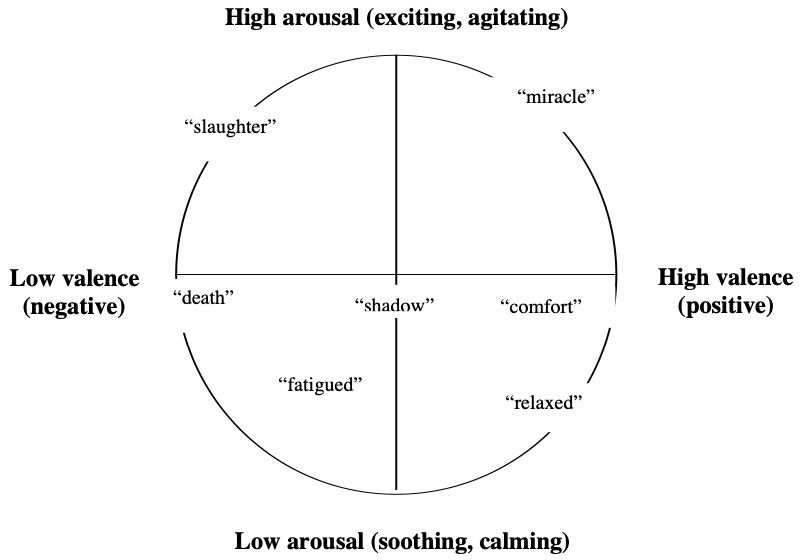
\includegraphics[scale=0.75]{va_plane.png} 
	\caption{Valence and arousal plane, described in \cite{kensinger2004remembering}}
    \label{fig:va_plane}
\end{figure}
High arousal emotional events are encoded better that non-arousing events. Instead of increasing overall attention to an event, an emotionally arousing stimulus decreased attentional resources available for information processing and focused attention only on the arousal-eliciting stimulus.
\\ \indent
The experience of music listening is multidimensional. Different emotions are associated with different music patterns. For example, arousal is associated to:
\begin{itemize}
	\item tempo (fast/slow)
	\item pitch (high/low)
	\item loudness (high/low)
	\item timbre (bright/soft)
\end{itemize}
while valence is associated to:
\begin{itemize}
	\item mode (major/minor)
	\item harmony (consonant/dissonant)
\end{itemize}
as expressed in \cite{gabrielsson2001influence}. Emotion perception is correlated to the combination of music factor, rarely from just one of them. For example, loud chords and high-pitched chords tends to be feel as more positive valence than soft chords and low-pitched chords.





 
	\chapter{Theoretical Background on EDA}
\label{chap:TheoreticalBackgroundEDA}
\pagestyle{plain}
\vspace{0.5cm}

\noindent This chapter introduces the readers to Electrodermal Activities and how are they related with Music Emotion Recognition task.

\section{Electrodermal phenomena}
Already in the 80's, psychological factors related to electrodermal phenomena were observed. It became an important field of study, due to the fact its ease of obtaining a distinct \gls{edr}, the intensity of which seems apparently related to stimulus intensity and/or its psychological significance \cite{boucsein2012electrodermal}.
\\ \indent
While there is still widespread disagreement and confusion about the nature and causes of musically evoked emotions, recent studies involving real-time observation of brain activity seem to show that areas of the brain linked with emotion (as well as pleasure and reward) are activated by music listening \cite{trost2012mapping}.

\section{Electrodermal Activity}
\gls{eda} was first introduced by Johnson and Lubin in 1966 \cite{johnson1996} as a common term for all electrical phenomena in skin, including all active and passive electrical properties that can be traced back to the skin and its appendages.
\\
\gls{eda} is the property of the human body that causes continuous variation in the electrical characteristics of the skin. Historically, \gls{eda} has also been known as \gls{sc}, \gls{gsr}, \gls{edr}, \gls{pgr}, \gls{scr}, \gls{ssr} and \gls{scl}. The long history of research into the active and passive electrical properties of the skin by a variety of disciplines has resulted in an excess of names, now standardized to \gls{eda}.
\\ \indent
The use of the term \textit{response} for phasic electrodermal phenomena suggests that there is a distinct relationship to a stimulus producing an \gls{edr}. Sometimes there are phasic parts that cannot be traced to any specific simulation, they are called \textit{spontaneous} or \textit{non-specific} \gls{edr}.
\\ \indent
There is ample empirical evidence that electrodermal phenomena are generated by sweat gland activity in conjunction with epidermal membrane processes. When sweat gland activity is abolished in humans, either as a result of congenital absence, by sympathectomy, by peripheral sudomotor nerve discharge, or by pharmacological blocking, \gls{scr} and SPRs are normally eliminated and \gls{scl} is considerably reduced \cite{fowles1993electrodermal}.
\\ \indent
As mentioned before, skin conductance is characterized by:
\begin{itemize}
	\item Tonic also called \gls{scl}, smooth underlying slowly changing level, it accounts for the general levels of the coductivity of the skin.
	\item Phasic, \gls{scr} rapidly changing peaks, results from momentary sympathetic activation when arousing stimuli are present.
\end{itemize}
In the figure \ref{fig:signal_phasic} can be seen an \gls{eda} file plot and the division in Tonic and Phasic parts thanks to \href{https://github.com/MPBA/pyphysio}{pyphysio}\footnote{https://github.com/MPBA/pyphysio} library \cite{bizzego2019pyphysio}.
%\begin{figure}[h]
%    \centering
%    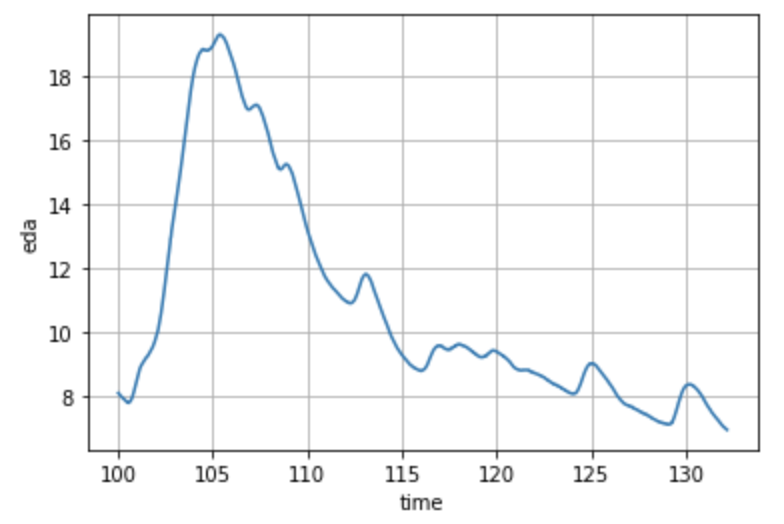
\includegraphics[scale=0.75]{eda_graph.png} 
%	\caption{Graph of an EDA signal plot thanks to \cite{bizzego2019pyphysio} library}
%    \label{fig:eda_graph}
%\end{figure}
\begin{figure}[h]
    \centering
    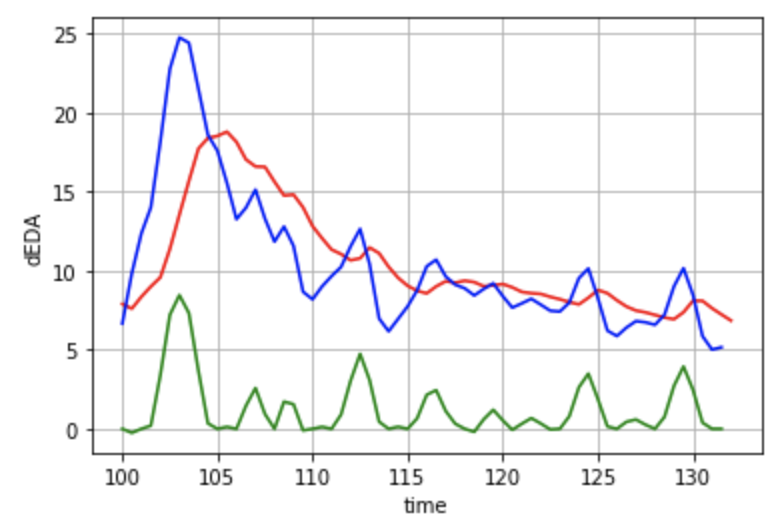
\includegraphics[scale=0.8]{signal_phasic.png} 
	\caption{Representation EDA signal (in red), driver signal (in blue) and phasic signal (in green)}
    \label{fig:signal_phasic}
\end{figure}
\\
Another useful graph is shown in the figure \ref{fig:phasic_tonic} from \cite{hernandez2014using} that represent division between the complete signal (in blue), the tonic component (in dashed green) and the phasic component (in red).
\begin{figure}[h]
    \centering
    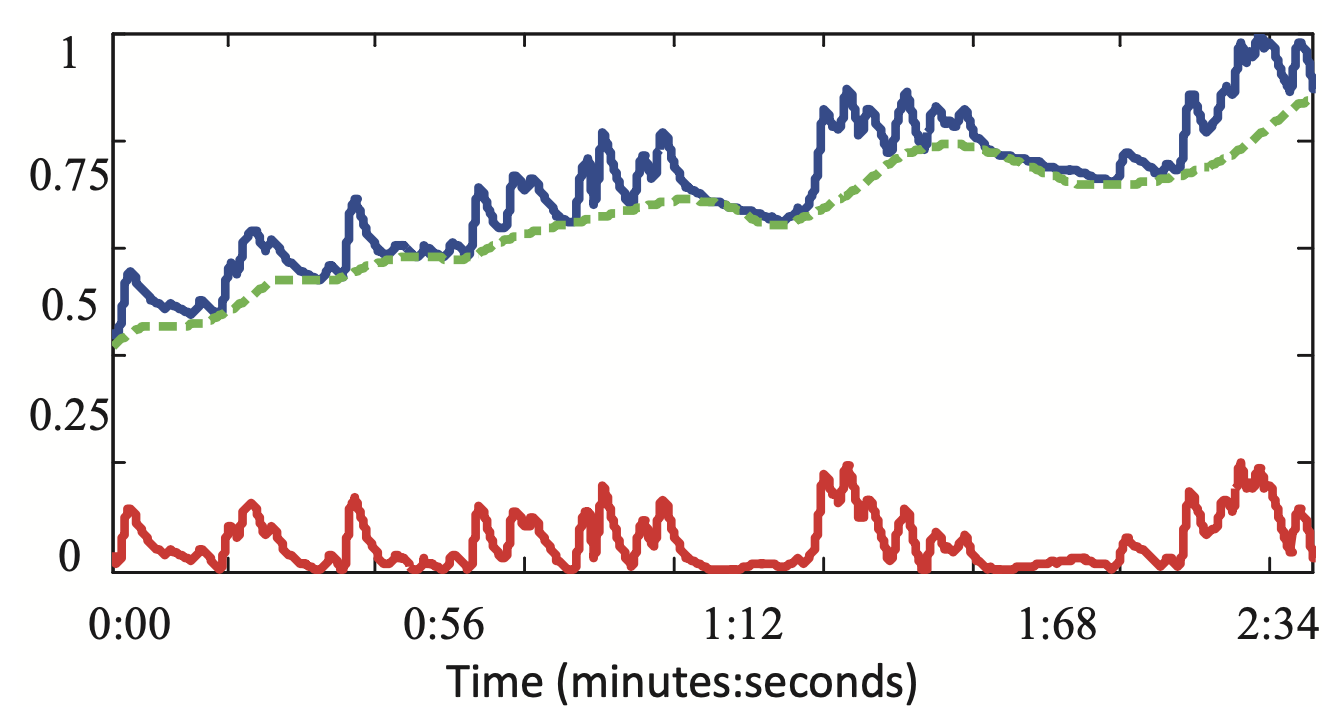
\includegraphics[width=0.8\textwidth]{phasic_tonic.png} 
	\caption{Representation of EDA signal (in red), driver signal (in blue) and phasic signal (in dashed green) from \cite{hernandez2014using}}
    \label{fig:phasic_tonic}
\end{figure}
\\
The time series of the change of \gls{sc} can be characterized by a slowly varying tonic activity and fast varying phasic activity. The \gls{scr} shows a steep incline to the peak and a slow decline to the basilne. The successions of \gls{scr} usually results in a superposition of subsequent \gls{scr} as one \gls{scr} arises on top of the declining trail of the preceding one.
\\
The figure \ref{fig:skin_conductance} from \cite{benedek2010continuous} shows a \gls{sc} data section, the upper row shows the original \gls{sc} data. The middle row shows the driver signal which results from deconvolution of the \gls{sc} data. Inter-impulse data are used to estimate the tonic part of the driver at 10-s intervals (tonic grid points). The tonic driver is used to compute the tonic \gls{sc} (see upper row). Subtraction of the tonic part from the driver results in the phasic driver (lower row). The phasic driver shows a virtually zero baseline and distinct phasic responses. 
\begin{figure}[h]
    \centering
    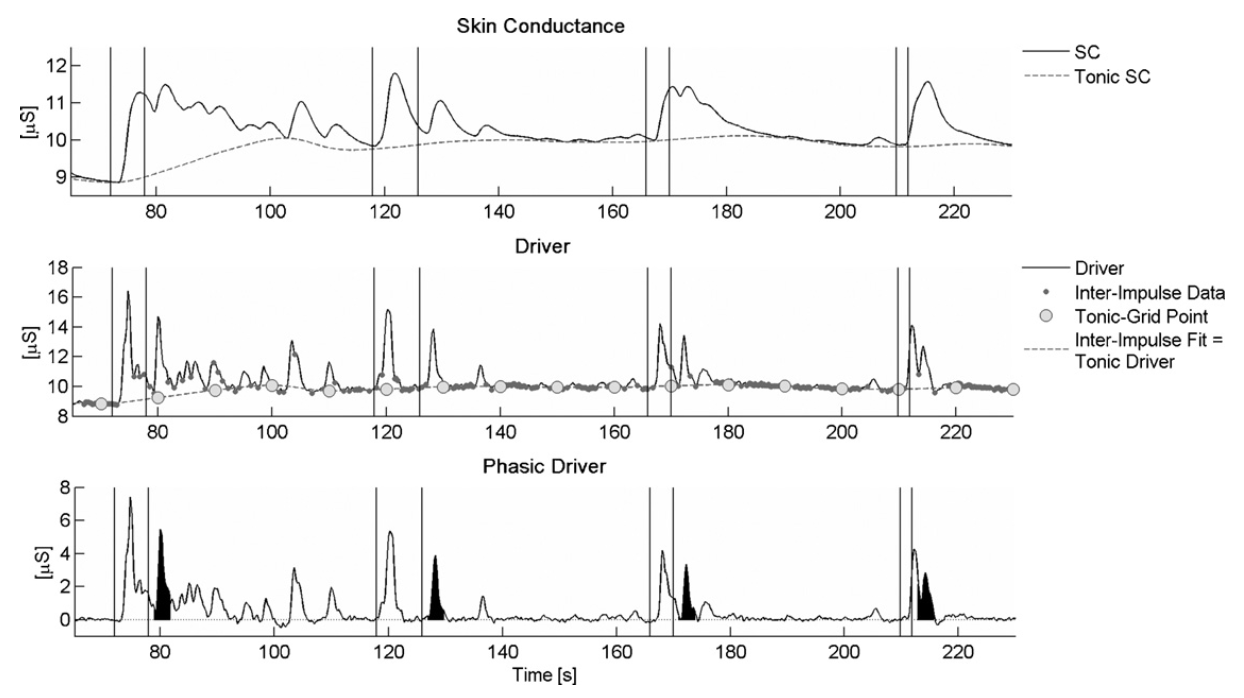
\includegraphics[width=\textwidth]{skin_conductance.png} 
	\caption{Skin conductance and phasic driver extraction from \cite{benedek2010continuous}}
    \label{fig:skin_conductance}
\end{figure}

\subsection{Measurement principles}
\gls{eda} can be measured both without externally applied voltage (endosomatic method) or with application of \gls{dc} or \gls{ac} (exosomatic method). The widespread used method is the exosomatic with \gls{dc} recordings. With direct voltage, skin resistance measurements will result when current is constant, while skin conductance measurement will result when voltage is kept constant.
\\ \indent
There are some factors that should be controlled as possible sources or variance in \gls{eda} recordings, like environmental conditions as the climatic conditions and physiological factors like age, gender and ethnic differences.
\\ \indent
\gls{eda} can be measured in many different ways electrically including skin potential, resistance, conductance, admittance, and impedance. It achieves this by passing a minuscule amount of current between two electrodes in contact with the skin. The units of measurement for conductance are microSiemens ($\mu$S).

\subsection{Recording techniques}
Electrodermal recording is usually performed with two electrodes. Exosomatic techniques use two active sites, while endosomatic recording requires an active and an inactive site.
\\
Figure \ref{fig:electrode_sites} illustrate the preferred palmar recording areas for exosomatic and endosomatic \gls{eda} recordings. Sites A and B for bipolar recordings. C and D for volar electrode sites.
\begin{figure}[h]
    \centering
    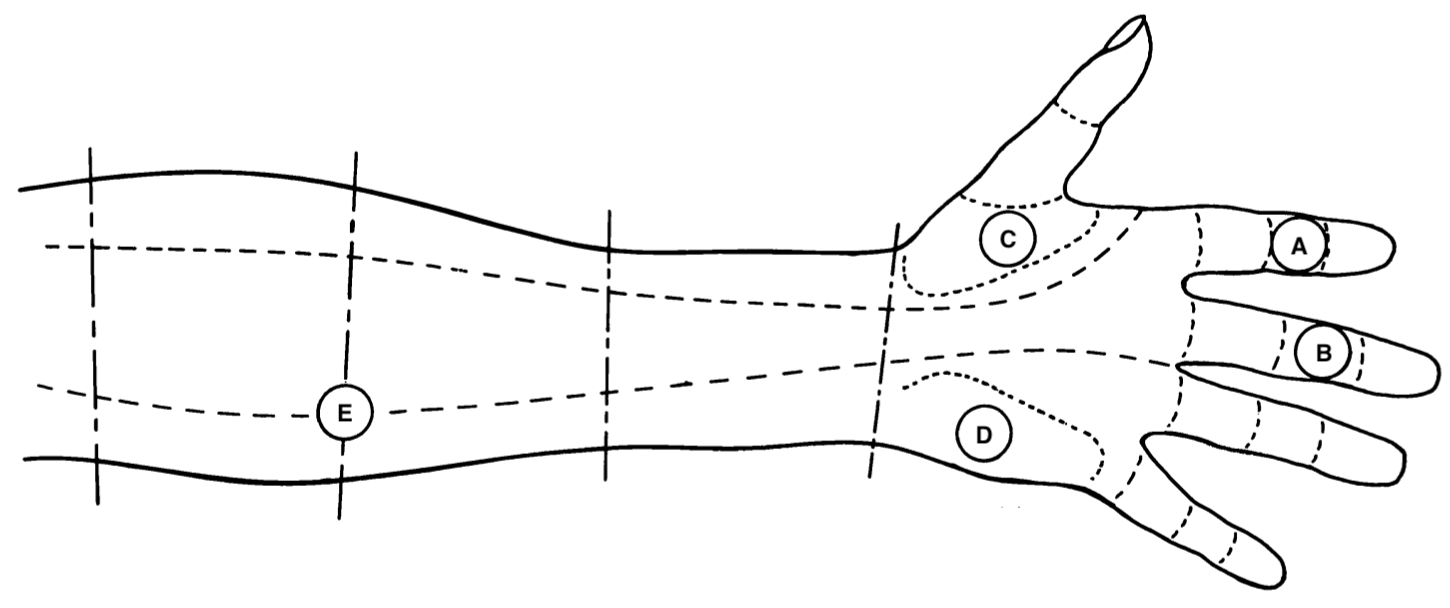
\includegraphics[width=\textwidth]{electrode_sites.png} 
	\caption{Preferred palmar recording areas for exosomatic and endosomatic EDA recordings}
    \label{fig:electrode_sites}
\end{figure}

\subsection{Artifacts identification in EDA data}
\gls{eda} data is often captured by wearable devices, which makes the signal collected vulnerable to several types of noise. Artifacts can be generated from electronic noise or variation in the contact between the skin and the recording electrode caused by pressure, excessive movement or adjustment of the device \cite{taylor2015automatic}.
\\
They may be mistaken for a skin conductance response, and this must be avoided.
\\ \indent
Typically, as Boucsein \cite{boucsein2012electrodermal} report, the shape of an \gls{scr} typically lasts between $1s$ to $5s$, has a steep onset and an exponentially decay and reaches an amplitude of at least $0.01\mu S$. An example of a typical \gls{scr} in figure \ref{fig:SCR_example}.
\begin{figure}[h]
    \centering
    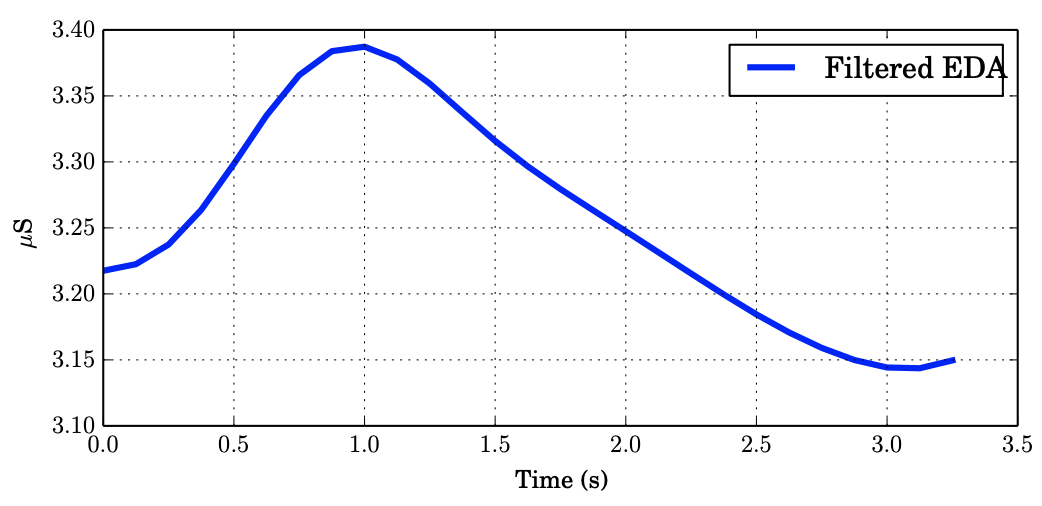
\includegraphics[scale=0.4]{SCR_example.png} 
	\caption{Example of a SCR shape}
    \label{fig:SCR_example}
\end{figure}
\\
Currently, many researchers deal with signal artifacts and noise by applying exponential smoothing or low-pass filtering.
\\
Additionally, filter cutoff frequencies are based only loosely on prior knowledge of typical characteristics of SCR shape, and vary widely study to study ($1Hz$ and $5Hz$). The cutoff frequency ultimately chosen for a study is specific to that particular study, making generalization difficult.
\\ \indent
There are much relevant techniques that are also able to recognize and compensate for large-magnitude artifacts that can result from pressure or movement of the device during recordings.
\\
In \cite{taylor2015automatic} is presented a figure reported at figure \ref{fig:eda_artifacts}, which shows a portion of signal that contains three artifacts, in which the fast decrease could not be produced by human physiology. Comparing the raw signal and the filtered version, the low-pass filter has not removed the artifacts.
\begin{figure}[h]
    \centering
    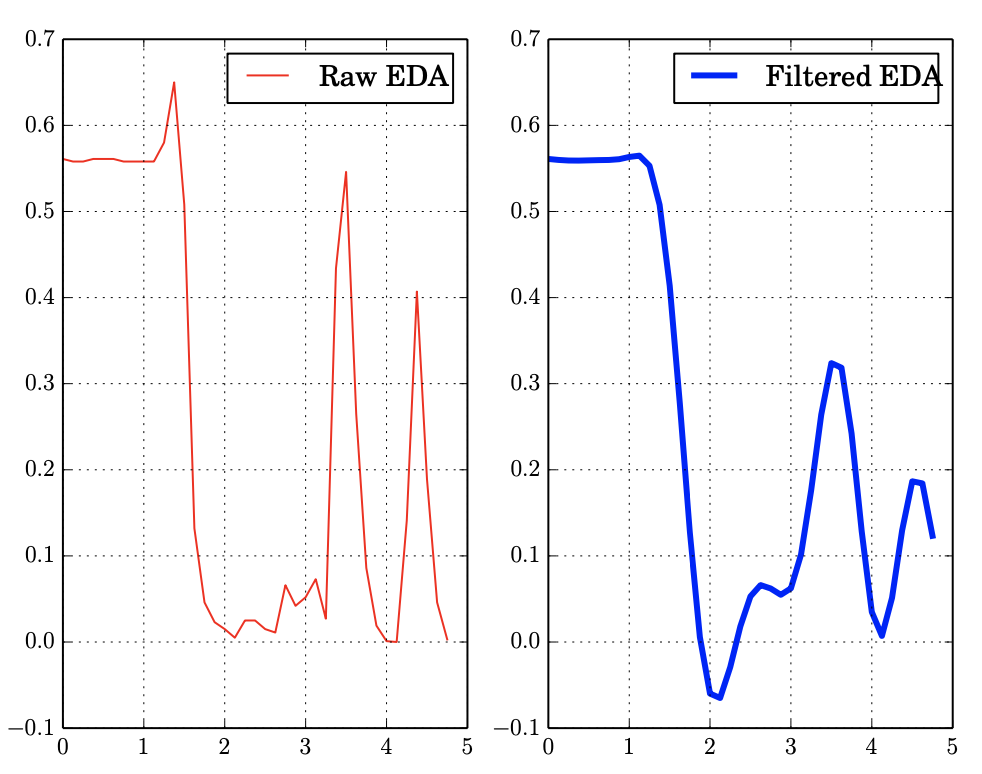
\includegraphics[scale=0.4]{eda_artifacts.png} 
	\caption{Portion of an EDA signal, the raw signal on the left in red, a $1Hz$ low-pass filter applied on the signal to the left in blue in \cite{taylor2015automatic} }
    \label{fig:eda_artifacts}
\end{figure}
\\
Some researchers, as Boucsein analysis \cite{boucsein2012electrodermal}, develop heuristic techniques for removing atypical portion of the \gls{eda} signal. Someone decide to discard portion of their data where the signal increased more than 20\% per second or decreased more than 10\% per second.
\\
In another case, a study which collected \gls{eda} from two sensors (on both the ankle and wrist) \cite{hedman2010situ} was able to detect artifacts by looking for epochs when only one of the two sensors had an abnormally low signal, or showed an unusually rapid increase or decrease.
\\ \indent
In \cite{taylor2015automatic} developed a \gls{ml} algorithm for automatically detecting \gls{eda} artifacts, providing empirical evaluation of classification performances.

\subsection{EDA features}
As for \gls{mer} analysis, also in \gls{eda} data analysis, is important to find which features need to be extracted and than which feature selection method must be carried.
\\ \indent
Emotion recognition from \gls{eda} has been commonly used for the assessment of user's experience in a variety of contexts such as recreational and games \cite{drachen2010correlation} and driving \cite{healey2005detecting}. Previous research has explored the predictive power of a diverse set of \gls{eda} features of different types, including time domain, frequency domain, and time-frequency domain features.
\\ \indent
Regarding time domain features, most usually features considered are the statistical parameters of the signal as:
\begin{itemize}
	\item Mean value: $\mu$ is the central value of a discrete set of numbers $x_1,x_2,...,x_n$, specifically, the sum of the values divided by the number of values:
		\begin{equation}
		\mu=\dfrac{1}{n} \sum_{i=1}^{n}{x_i}
		\end{equation}
	\item Standard deviation:  is a measure of the amount of variation or dispersion of a set of values:
		\begin{equation}
		\sigma=\sqrt{\dfrac{1}{n}\sum_{i=1}^{n}({x_i-\mu})^2}
		\end{equation}
	\item Kurtosis: is a measure of the "tailedness" of the probability distribution of a real-valued random variable:
		\begin{equation}
		kurt=\dfrac{\dfrac{1}{n} \sum_{i=1}^{n}{(x_i-\mu)^4}}{\sigma^4}
		\end{equation}
	\item Skewness: is a measure of the asymmetry of the probability distribution of a real-valued random variable about its mean:
		\begin{equation}
		skew=\dfrac{\dfrac{1}{n} \sum_{i=1}^{n}{(x_i-\mu)^3}}{\sigma^3}
		\end{equation}
\end{itemize}
In \cite{shukla2019feature}, as an example, were extracted the features for \gls{eda} data shown in table \ref{table:features}, where \gls{dwt} is an implementation of the wavelet transform using a discrete set of wavelet scales.
\begin{table}[h!]
	\centering
	\begin{tabular}{|l |p{0.36\textwidth} | p{0.3\textwidth}|}
		\hline
		Domain & Feature vector & Number of features\\ [0.5ex] 
		\hline\hline Time & \gls{scr} related \newline Statistical features \newline Hjorth features \newline Higher Order Crossing & 7 \newline 8 \newline 2 \newline 5 \\ 
		\hline	Frequency	 & Statistical features \newline Band power & 8 \newline 9 \\ 
		\hline	Time-Frequency & \gls{dwt} coefficients \newline SWT features \newline \gls{mfcc} \newline Statistical features \gls{mfcc} & 56 \newline 40 \newline 481 \newline 5 \\
		\hline
	\end{tabular}
	\caption{Features extracted in \cite{shukla2019feature}}
	\label{table:features}
\end{table}
\\
Other cases, researchers have focused on event-related features of \gls{eda}. They are useful when are presented to the subjects some events, stimulus, like images or sounds.
\\
Examples of event-related aspects of \gls{eda} considered in other studies are \gls{scr} amplitude, \gls{scr} peak count, mean \gls{scr} rise time, or the sum of \gls{scr} areas.
\\ \indent
Fewer researches, as \cite{shukla2019feature} remarks, has focused on the predictive power of \gls{eda} related to the frequency domain. The frequency domain analysis has shown superior capability for the gradient component's detection of individual \gls{scr}.
\\
Due to the different rate of physiological process, \gls{eda} signals vary significantly with the frequency \cite{ghaderyan2016efficient}.
\\
Frequency oscillations of \gls{eda} signals can be divided into different frequency sub-bands to analyze it. Indeed previous researchers has considered statistical aspects.
\\ \indent
As for audio, also for \gls{eda} data, after constructing a feature matrix, need to apply an algorithm of feature selection to improve data reliability.
\\ \\
Some examples of feature selection could be:
\begin{itemize}
	\item \gls{jmi}: focuses on the increasing complementary information between features.
	\item \gls{cmim}: it can properly identify truly redundant features and noisy features, and gives preference to informative, uncorrelated features.
	\item \gls{disr}: a normalized variant of \gls{jmi}.
\end{itemize}
In general it is not known which features are most appropriate for emotion recognition from \gls{eda} and previous works have made limited contributions on a systematic comparison of \gls{eda} features.
\\
In \cite{shukla2019feature} there is a table showing various features extracted for \gls{eda} signals already presented in table \ref{table:features} with also references in the literature.
	\chapter{State of the Art}
\label{chap:StateOfTheArt}
\pagestyle{plain}
\vspace{0.5cm}

\noindent This chapter introduces the readers to a complete review of the problem and all the different resolution possibilities.

\section{Physiological signals}
In this section will be defined a general overview on physiological signals that can be used in order to achieve a solution to the Music Emotion Recognition problem.
\\ \indent
Emotions, which affect both human physiological and psychological status, play a very important role in human life. Positive emotions help improve human health and work efficiency, while negative emotions may cause health problems. Long term accumulations of negative emotions are predisposing factors for depression, which might lead to suicide in the worst cases.
\\
The emotion often refers ti a mental state that arises spontaneously rather than through conscious effort and it is accompanied by physical and physiological changes, relevant to the human organs and tissues such as brain, heart, skin, blood flow, muscle, facial expressions, voice, etc. \cite{shu2018review}.
\\ \indent
Emotion recognition has been applied in many areas such as safe driving \cite{de2016enhancing}, health care especially mental health monitoring \cite{guo2013pervasive}, social security \cite{verschuere2006psychopathy}, and so on.
\\
In general, emotion recognition methods could be classified into two major categories:
\begin{itemize}
	\item Using human physical signals such as facial expression \cite{zhang2016facial}, speech \cite{mao2014learning}, gesture, posture, etc. This method has the advantage of easy collecting and is a chapter which has been studied for years. On the other side, the reliability cannot be guaranteed, as it is relatively easy for people to control the physical signals like facial expression or speech to hide real emotions, especially during social communications.
	\item Using internal signals as:
	\begin{itemize}
		\item Electroencephalogram (EEG)
		\item Electrocardiogram (ECG)
		\item Electromyogram (EMG)
		\item Blood Pressure (BP)
		\item Hearth Rate Variability (HRV)
		\item Electrodermal Activity (EDA) as:
		\begin{itemize}
			\item Skin Resistance (SR)
			\item Skin Temperature (ST)
			\item Skin Conductivity (SC)
			\item Galvanic Skin Response (GSR)
		\end{itemize}
		\item Respiration (RSP)
	\end{itemize}
	These signals are produced by the Nervous System which is divided into:
	\begin{itemize}
		\item Central Nervous System (CNS)
		\item Peripheral Nervous System (PNS): consist of the autonomic and somatic nervous systems (ANS and SNS).
	\end{itemize}
	EEG, ECG, EMG, GSR, RSP and GSR change in a certain way when people face some specific situations. Physiological signals are in response to the CNS and ANS. Due to the fact that CNS and ANS are involuntarily activated, they cannot be controlled.
\end{itemize}
In the table \ref{table:biological_signals} is shown a summary of various papers using different biological signals.
\begin{table}[h!]
	\centering
	\begin{tabular}{|l|l|}
		\hline
		Biological signal & Paper\\ [0.5ex] 
		\hline \hline ECG & \cite{dissanayake2019ensemble}, \cite{hsu2017automatic},  \cite{naji2014classification}, \cite{naji2015emotion}, \cite{cai2009research}  \\ 
		\hline ECG, EMG, RSP & \cite{kim2008emotion} \\
		\hline ECG, GSR & \cite{goshvarpour2017accurate} \\ 
		\hline HR, SR & \cite{yoo2005neural} \\
		\hline EEG & \cite{sourina2012real} \\
		\hline HR & \cite{nardelli2015recognizing} \\
		\hline
	\end{tabular}
	\caption{Papers with correspondent biological signal used}
	\label{table:biological_signals}
\end{table}
\newpage
In table \ref{table:physiological_features_relation} is presented the relationship between emotions and physiological features, thanks to \cite{shu2018review}. Arrows indicate increased ($\uparrow$), decreased ($\downarrow$), no change in activation from the baseline ($-$) or both increases and decreases in different studies ($\uparrow\downarrow$).
\begin{table}[h!]
\begin{adjustwidth}{-3cm}{-1cm}
	\centering
	\begin{tabular}{|c|c|c|c|c|c|c|c|}
		\hline
		Signal & Anger & Anxiety & Embarrassment & Fear & Amusement & Happiness & Joy\\ [0.5ex] 
		\hline \hline \textbf{Cardiovascular} &&&&&&& \\ 
		\hline HR & $\uparrow$ & $\uparrow$ &  $\uparrow$ & $\uparrow$ & $\uparrow\downarrow$ & $\uparrow$ & $\uparrow$ \\
		\hline HRV & $\downarrow$ & $\downarrow$ & $\downarrow$ & $\downarrow$ & $\uparrow$ & $\downarrow$ & $\uparrow$ \\
		\hline LF & & $\uparrow$ & & $(-)$ & & $(-)$ & \\
		\hline LF/HF & & $\uparrow$ & & & $(-)$ & & \\
		\hline PWA & & & & $\uparrow$ & & & \\
		\hline PEP & $\downarrow$ & & $\downarrow$ & $\downarrow$ & $\uparrow$ & $\uparrow$ & $\uparrow\downarrow$ \\
		\hline SV & $\uparrow\downarrow$ & $(-)$ & & $\downarrow$ & & $(-)$ & $\downarrow$\\
		\hline CO & $\uparrow\downarrow$ & $\uparrow$ & $(-)$ & $\uparrow$ & $\downarrow$ & $(-)$ & $(-)$ \\
		\hline SBP & $\uparrow$ & $\uparrow$ & $\uparrow$ & $\uparrow$ & $\uparrow$ & $\uparrow$ & $\uparrow$ \\
		\hline DBP & $\uparrow$ & $\uparrow$ & $\uparrow$ & $\uparrow$ & $\uparrow$ & $\uparrow$ & $(-)$\\
		\hline MAP & & & $\uparrow$ & $\uparrow$ & $\uparrow$ & $\uparrow$ & \\
		\hline TPR & $\uparrow$ & & & $\downarrow$ & $\uparrow$ & $\uparrow$ & $(-)$ \\
		\hline FPA & $\downarrow$ & $\downarrow$ & & $\downarrow$ & $\downarrow$ & $\uparrow\downarrow$ & \\
		\hline FPTT  & $\downarrow$ & $\downarrow$ & & $\downarrow$ & & $\uparrow$ & \\
		\hline EPTT & & $\downarrow$ & & $\downarrow$ & & $\uparrow$ & \\
		\hline FT  & $\downarrow$ & $\downarrow$ & & $\downarrow$ & $(-)$ & $\uparrow$ &\\
		\hline \hline \textbf{Electrodermal} &&&&&&& \\ 
		\hline SCR & $\uparrow$ & $\uparrow$ & & $\uparrow$ & $\uparrow$ & & \\
		\hline nSRR & $\uparrow$ & $\uparrow$ & & $\uparrow$ & $\uparrow$ & $\uparrow$ & $\uparrow$ \\
		\hline SCL & $\uparrow$ & $\uparrow$ & $\uparrow$ & $\uparrow$ & $\uparrow$ & $\uparrow$ & $(-)$ \\
		\hline \hline \textbf{Respiratory} &&&&&&& \\ 
		\hline RR & $\uparrow$ & $\uparrow$ & & $\uparrow$ & $\uparrow$ & $\uparrow$ & $\uparrow$ \\
		\hline Ti & $\downarrow$ & $\downarrow$ & & $\downarrow$ & $\downarrow$ & $\downarrow$ & \\
		\hline Te & $\downarrow$ & $\downarrow$ & & $\downarrow$ & & $\downarrow$ & \\
		\hline Pi & $\uparrow$ & & & $\uparrow$ & & $\downarrow$ & \\
		\hline Ti/Ttot & & & & $\uparrow$ & $\downarrow$ & & \\
		\hline Vt & $\uparrow\downarrow$ & $\downarrow$ & & $\uparrow\downarrow$ & $\uparrow\downarrow$ & $\uparrow\downarrow$ & \\
		\hline Vi/Ti & & & & & & $\uparrow$ & \\
		\hline \hline \textbf{Electroencephalography} &&&&&&& \\ 
		\hline PSD($\alpha$ wave) & $\uparrow$ & $\uparrow$ & & $\downarrow$ & $\uparrow$ & $\uparrow$ &  $\uparrow$ \\
		\hline PSD($\beta$ wave) & $\downarrow$ & & & & $\uparrow$ & & \\
		\hline PSD($\gamma$ wave) & & & & $\downarrow$ & $\uparrow$ & $\uparrow$ & $\uparrow$ \\
		\hline DE (avg) & $\uparrow$ & $(-)$ & & $\downarrow$ & & $\uparrow$ & $\uparrow$ \\
		\hline DASM (avg) & $(-)$ & & & $\uparrow$ & $\downarrow$ & $\downarrow$ & $\downarrow$ \\
		\hline RASMs (avg) & $\uparrow$ & & & $\uparrow$ & & $\downarrow$ & \\
		\hline
	\end{tabular}
	\end{adjustwidth}
	\caption{Relationship between emotions and physiological features}
	\label{table:physiological_features_relation}
\end{table}
\newpage
The position of different biosensors is shown in figure \ref{fig:biosensors_position}.
\begin{figure}[h]
    \centering
    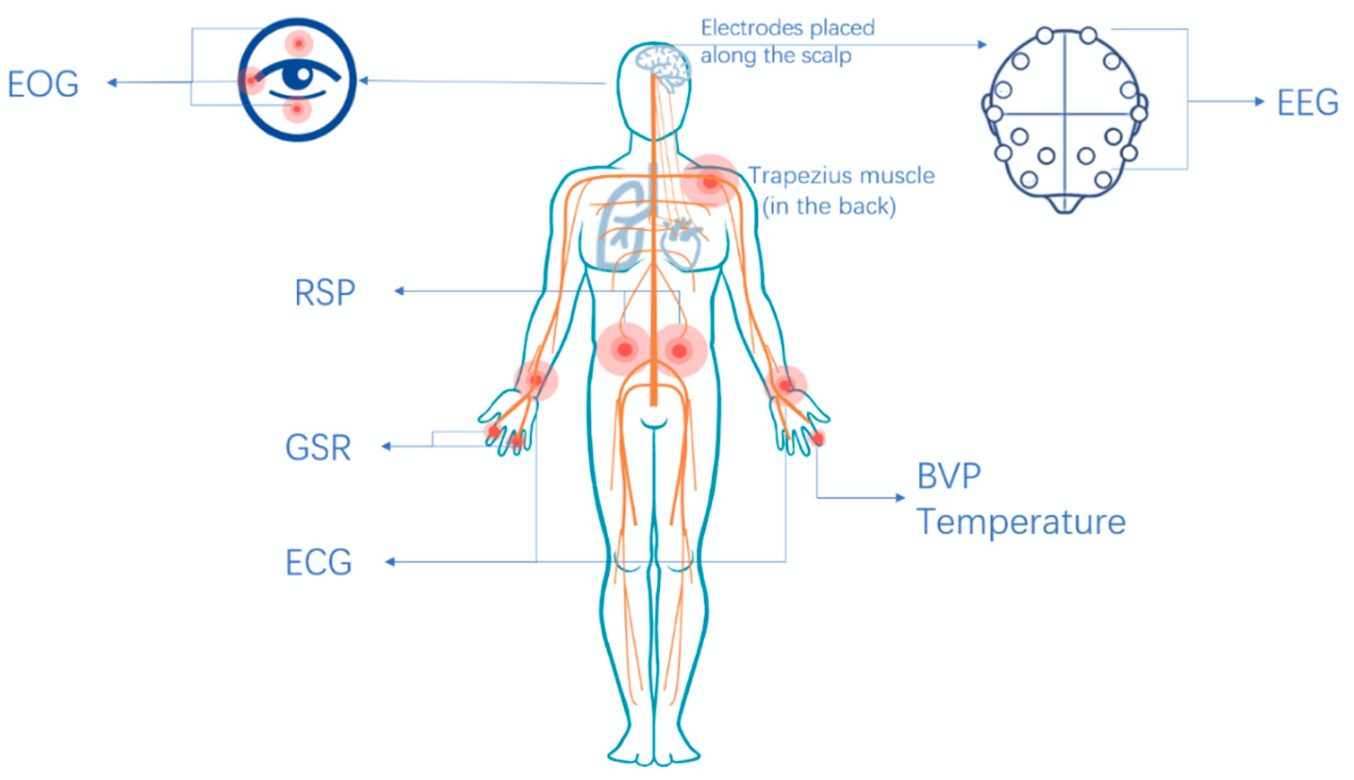
\includegraphics[width=0.8\textwidth]{biosensors_position.png} 
	\caption{Position of the bio-sensors}
    \label{fig:biosensors_position}
\end{figure}

\subsection{Electroencephalogram}
Electroencephalogram (EEG) is an electrophysiological monitoring method to record electrical activity of the brain. EEG measures voltage fluctuations resulting from ionic current within the neurons of the brain. Clinically, EEG refers to the recording of the brain's spontaneous electrical activity over a period of time, as recorded from multiple electrodes placed on the scalp.
\\ \indent
EEG is most often used to diagnose epilepsy, which causes abnormalities in EEG readings.[2] It is also used to diagnose sleep disorders, depth of anesthesia, coma, encephalopathies, and brain death.
\\ 
Many studies have indicated that the physiological correlates of emotions are likely to be found in the central nervous system rather than simply in peripheral physiological responses. Researchers have supported this viewpoint using EEG or other neuroimaging (e.g., functional Magnetic Resonance Imaging) approaches to investigate the specificity of brain activity associated with different emotional states.
\\
However, most of the available studies on emotion-specific EEG response have focused on EEG characteristics at the single-electrode level, rather than at the level of EEG-based functional connectivity.

\subsection{Electrocardiogram}
Electrocardiogram (ECG) is a recording of the electrical activity of the hearth using electrodes placed on the skin. These electrodes detect small electrical changes that are a consequence of cardiac muscle depolarization followed by repolarization during each cardiac cycle, the heartbeat.
\\ \indent
There are three main components to an ECG: the P wave, which represents the depolarization of the atria; the QRS complex, which represents the depolarization of the ventricles; and the T wave, which represents the repolarization of the ventricles, as in figure \ref{fig:ECG}.
\begin{figure}[h]
    \centering
    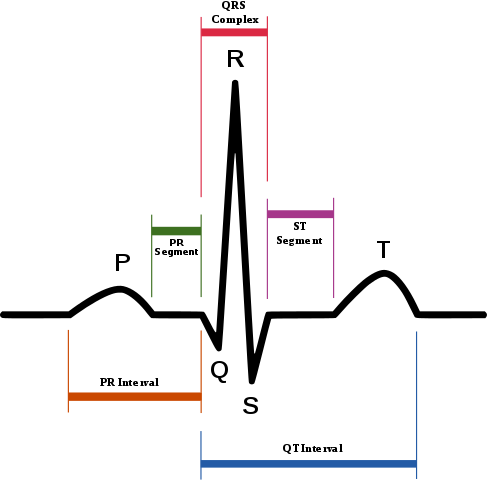
\includegraphics[width=0.6\textwidth]{ECG.png} 
	\caption{ECG of a heart in normal sinus rhythm}
    \label{fig:ECG}
\end{figure}

\subsection{Electromyogram}
Electromyogram (EMG) is an electrodiagnostic medicine technique for evaluating and recording the electrical activity produced by skeletal muscles.
\\
An electromyograph detects the electric potential generated by muscle cells when these cells are electrically or neurologically activated. The signals can be analyzed to detect medical abnormalities, activation level, or recruitment order, or to analyze the biomechanics of human or animal movement.
\\ \indent
Therefore, the best readings are obtained when the sensor is placed on the muscle belly and its positive and negative electrodes are parallel to the muscle fibers. Since the number of muscle fibers that are recruited during any given contraction depends on the force required to perform the movement, the intensity (amplitude) of the resulting electrical signal is proportional to the strength of contraction.
\\ \indent
In psychophysiology, EMG was often used to find the correlation between cognitive emotion and physiological reactions. In the work by Sloan \cite{sloan2004emotion}, for example, the EMG was positioned on the face (jaw) to distinguish \textit{smile} and \textit{frown} by measuring the activity of zygomatic major and corrugator supercilli. In experiment of \cite{kim2008emotion}, bipolar electrodes were placed at the upper trapezius muscle (near the neck) in order to measure the mental stress of the subjects.

\subsection{Hearth Rate Variability}
Hearth Rate Variability (HRV) measure the beat-to-beat temporal changes of the hearth rate, sometimes it is calculated from ECG, but the usability of measuring the ECG is limited. HRV can be evaluatd also through the Blood Volume Pulse (BVP) or Photoplethysmography (PPG).
\\ \indent
A reduced HRV is linked to psychiatric illness as depression, anxiety. The heart rate is the most natural choice for arousal detection using comparison of sympathetic and parasympathetic frequency bands of the time series. However, it is highly dependent on the position of the body during monitoring.

\subsection{Electrodermal Activity}
As already been studied in chapter \ref{chap:TheoreticalBackgroundEDA}, EDA measures the resistance of the skin and the skin conductivity applying electrodes to the skin. The skin conductivity decreases during relaxed states, and increase when exposed to effort.

\subsection{Respiration}
Respiration (RSP) is the process of moving air into an out of the lungs to facilitate gas exchange with the internal environment, mostly bringing in oxygen and flushing out carbon dioxide.
\\
The respiration can be measured with a latex rubber band, the amount of stretch in the elastic is measured as a voltage change and recorded. The most common measures of RSP are the depth of breathing and the rate of RSP.
\\ \indent
RSP rate generally decreases with relaxation, tense situations may result in momentary RSP cessation. Irregularity in the RSP pattern could be the cause of negative emotions.
\\
Due to the fact that RSP is closely linked to the cardiac function, RSP can be affect other measures like EMG and SC measurements.
\\
Positions to the left, and typical waveform of the signals to the right are presented in the figure \ref{fig:waveform_biosensors}.
\begin{figure}[h]
    \centering
    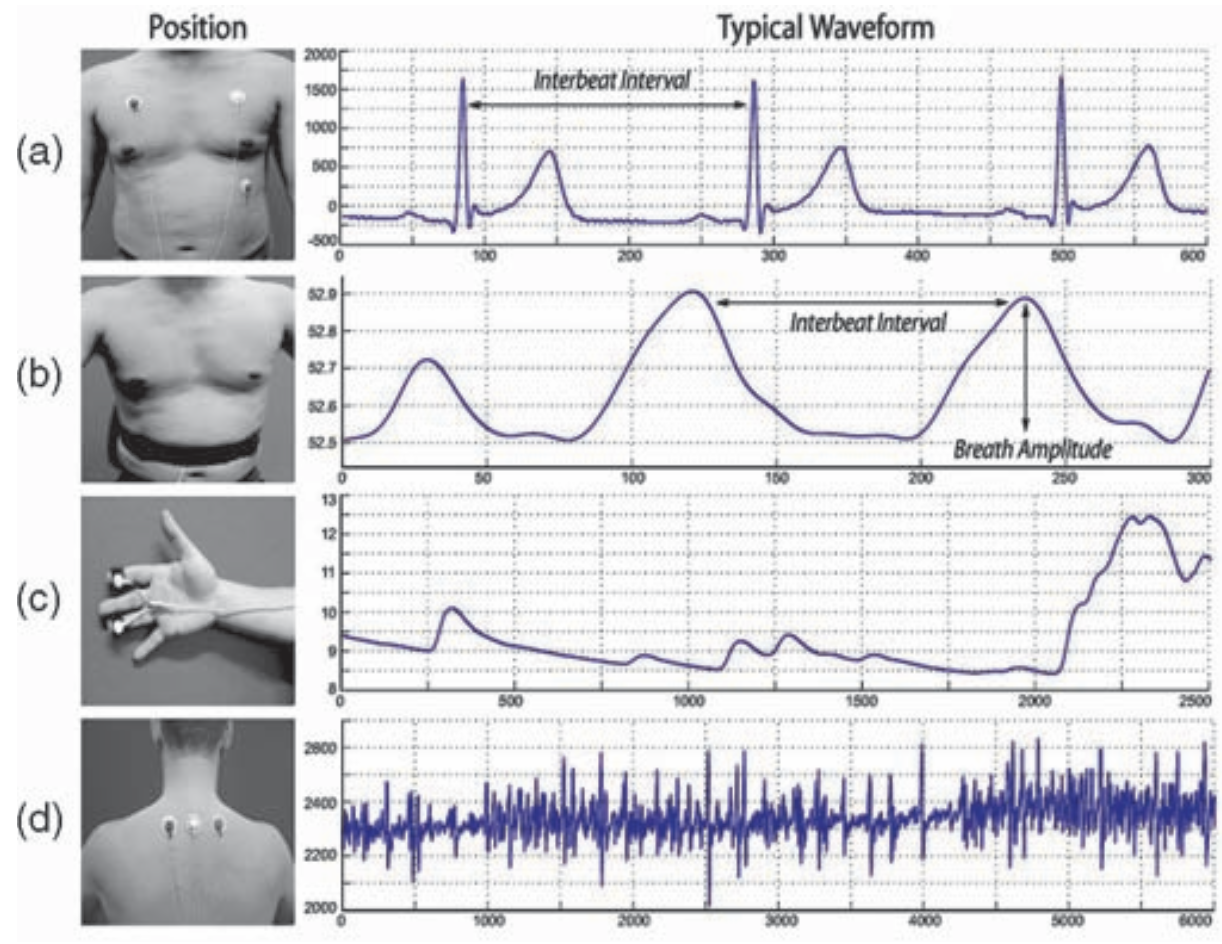
\includegraphics[width=0.8\textwidth]{waveform_biosensors.png} 
	\caption{Positions (left) and waveform of the signals (right), (a) ECG, (b) RSP, (c) SC, (d) EMG}
    \label{fig:waveform_biosensors}
\end{figure}

\section{General methodology}
For physiological signal-based emotion recognition, there is a common methodology which can be divided into two categories:
\begin{itemize}
	\item Traditional Machine Learning methods: model specific methods, which require carefully designed hand-crafted features and feature optimization methods.
	\item Deep learning methods, model-free methods, which can learn the inherent principle of the data and extract features automatically.
\end{itemize}
The whole emotion recognition framework is shown in figure \ref{fig:emotion_recognition_process}.
\begin{figure}[h]
    \centering
    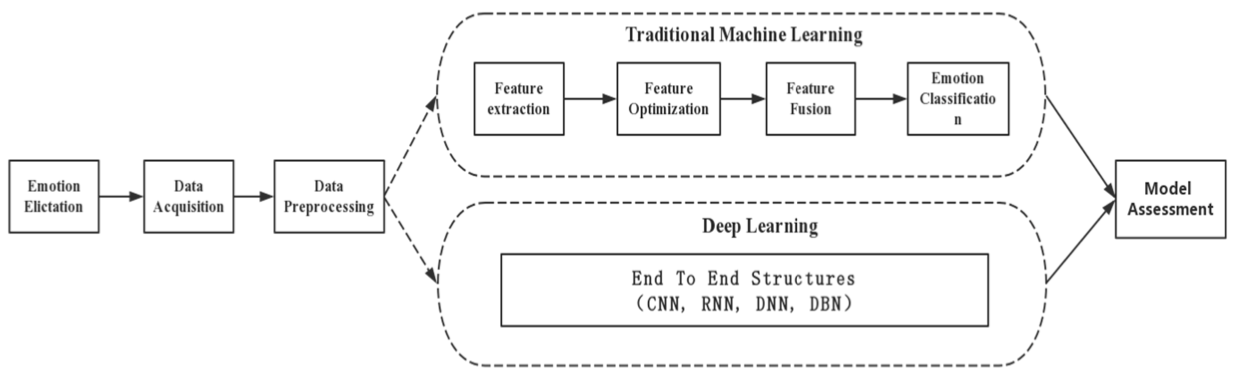
\includegraphics[width=\textwidth]{emotion_recognition_process.png} 
	\caption{Emotion recognition process using physiological signals under targer emotion stimulation}
    \label{fig:emotion_recognition_process}
\end{figure}

\subsection{Preprocessing}
After the part of data acquisition, which is different for each physiological signal, there is the data preprocessing step. It is necessary to eliminate the noise effect, artifacts and other signal parts that may lead to wrong results. Due to the complex and subjective nature of raw physiological signals and the sensitivity to noises, electromagnetic interferences, movement artifacts, ... this step is mandatory.
\\ \indent
Some of the common steps can be summarized in:
\begin{itemize}
	\item Filtering: is commonly used a low-pass filter to remove noises, or also adaptive bandpass filters to remove artifacts.
	\item Discrete Wavelet Transform (DWT): used to reduce the noise of physiological signals
	\item Independent Component Analysis (ICA): used to extract and remove respiration sinus arrhythmia from ECG.
	\item Empirical Mode Decomposition (EMD): used to remove the eye-blink from EEG.
\end{itemize}

\subsection{Traditional Machine Learning}
Main steps for traditional ML methods, as already presented in \ref{ML}. There are processes including feature extraction, feature selection and classification.

\paragraph{Feature extraction}
\mbox{} \\ \\ \indent
Feature extraction plays a fundamental role in the emotion recognition model. Several major features are extracted for each physiological signal, because is important to extract the most prominent features for emotion recognition. For example EEG is a complex and non-stationary signal, so some statistical features like Power Spectral Density (PSD) and Spectral Entropy (SE) are commonly used.
\\
Often are extracted statistical features as mean, standard deviation, Kurtosis, Skewness, entropy.
\\
However, each bio-signal has to be investigated separately as extracted features might vary in their usefulness for the classification of emotions.

\paragraph{Feature selection}
\mbox{} \\ \\ \indent
After the feature extraction process, there might be a quantity of features, some of which may be irrelevant, some that are probably correlated each other, there might be some redundant features.
\\
It lead to a long time of analyzing the features and train the model and it is easy to produce overfitting problem and another problem of sparse features, called \textit{curse of dimensionality}, which results in the decrease of the model performance.
\\
Some of the main feature selection algorithms are RfeliefF, MRmR, Sequential Backward Selection (SBS) and Sequential Forward Selection (SFS), PCA, ...
\\ \indent
In general there are several feature selection alforithms, some reduce the dimensionality by taking out some redundant or irrelevant featuresm other transform the original one into a new set of features. Performances of the feature selection algorithm depends on the classifier and the dataset, due to this, the perfect feature selection algorithm do not exist.

\paragraph{Classification}
\mbox{} \\ \\ \indent
In emotion recognition, the major task is to assign the input signal to one of the given class sets. There are several classification models like Linear Discriminant Analysis (LDA), k-Nearest Neighbor (kNN), Support Vector Machine (SVM), Random Forest (RF), ...

\subsection{Deep Learning}
Deep Learning (DL) methods have the benefits to be model-free methods, so they do not depends on the specific model considered.
\\
Examples of DL algorithms are Convolutional Neural Network (CNN), Recurrent Neural Network (RNN), ... Neural network in general are particular types of ML methods which have as fundamental unit the node, loosely based on the biological neuron. 
\\ \indent
The relevant aspect of DL is that it can learn the inherent principle of the data and extract features automatically, so there is no need to extract feature and select the most relevant ones, which could lead to a better generalization of the problem.

\subsection{Model assessment and selection}
The generalization error of the classifier can be evaluated by experiments, where a testing set should be used to test the ability of the classifier to classify the new samples, and the testing error on the testing set could be viewed approximately as the generalization error.
\\
The dataset is divided into two mutually exclusive sets, the training and the testing set. It is important to maintain the consistency of the data distribution as much as possible. In general, the experiment need to repeat several times with random division and then calculate the average value as the evaluation result.
\\ \indent
There is also k-fold crossing-validation. the initial sampling is divided into $K$ sub-samples. One sub-sample is used as the testing set and the other $K-1$ samples are used for training. Cross-validation is repeated K-times. Each sub-sample is validate once and the average result of K times is used as the final result. The most common is the 10-fold cross-validation.
\\ \indent
To evaluate the performance of the experiment there is the accuracy, which is the proportion of samples that are correctly classified to the total samples.

\section{Issues of physiological signals}
A lot of efforts have been made in revealing the relationships between explicit physiological signals and implicit psychological feelings. However, there are still several challenges in emotion recognition based on physiological signals:
\begin{itemize}
	\item Need a very well designed setup in order to obtain high quality physiological data. The standard setup is the standard lab setting with subjects with earphones  sit motionless in front of a screen where the emotion stimuli materials are played. This system is fixed, data are noiseless and stable, but the issue of obtaining genuine emotions which is dependent heavily on the emotion stimulated materials is hard to deal with it.
	\item The stimulus materials are artificially selected, labels of the materials are manually set, while for the same thing human emotions vary from each other, this may lead to a large deviation in the rating of the material. In \cite{muhl2011modality}, the author showed that different introduction ways led to different physiological responses.
	\item There is no still clear evidence that what feature combination of what physiological signal combinations are the most significantly relevant to emotion changes.
	\item For most studies, the number of subjects is small. Due to limited samples, the performance of the classifier with subjects who have not been trained would be poor. The clear efficient method is to include more subjects from different ages and backgrounds.
	\item Emotion perception and experience lead to strong differences.
	\item The reliability of facial expressions cannot be guaranteed sometimes.
\end{itemize}

\section{Related works}
In this section will be presented some works done during the last years on all physiological signals that tries to understand the relationship of physiology and human emotions.

\subsection{ECG and GSR signal emotion recognition}
In the work \cite{goshvarpour2017accurate} Electrocardiogram and Galvanic Skin Response of 11 healthy students were collecred while subjects were listening to emotional music clips. They extracted Matching Pursuit (MP) coefficients frin ECG and GSR signals.
\\ \indent
Than were calculated some statistical indices from the MP coefficients and three dimensionality reduction method were applied, PCA, LDA and Kernel PCA. These features were fed into the Probabilistic Neural Network (PNN) in subject-dependent and subject-independent modes.
\\ \indent
The PNN is feed with a feature vector in the input layer, is determined a distance between the input and the weight vector. Is calculated the summation of these contributions for each input class to yield the probability. Finally is selected the maximum of these probabilities by a competitive layer and assigned $1$ for that class and $0$ elsewhere.
\\ \indent
They achieved, using PCA, the highest recognition rate of 100\% for $\sigma = 0.01$.

\subsection{ECG sensors for human emotion recognition}
The research of \cite{dissanayake2019ensemble}, they suggest an ensamble learning approach for developing a machine learning model that can recognize four major human emotions (anger, sadness, joy and pleasure) incorporating ECG signals.
\\ \indent
As feature extraction method, the analysis combines four ECG signals techniques. Several ML methods have been applied to the model, the most accurate (with an accuracy of 70\% is achieved by using an Extra Tree Classifier (a variant of the Random Forest that introduce more variation in the ensemble).

\subsection{Automatic ECG emotion recognition}
In \cite{hsu2017automatic} is presented an automatic ECG-based emotion recognition algorithm. They recorded ECG signal from subjects and extracted some features from the signal from the time and frequency domain. Than performed an algoritm of feature selection, a sequential forward floating selection-kernel-based class separability-based.
\\
Valence and arousal and four types of of emotions are recognized using Least Square-Support Vector Machine recognizer. They gained a classification rate for positive/negative valence, high/low arousal, and four types of emotion classification tasks are 82.78\%, 72.91\%, and 61.52\%, respectively.

\subsection{Classification of music emotions with  forehead biosignals and ECG}
In the work of \cite{naji2014classification} to recognize music-induced emotions is used a fusion of three-channel forehead biosignals (left and right temporal channel and frontalis) and ECG. They employed two parallel SVM as arousal and valence classifiers.
\\ \indent
The inputs of the classifiers were obtained by applying a fuzzy-rough model feature evaluation criterion and sequential forward floating selection algorithm.
\\
The average classification accuracy was of 88.78\% (valence classification accuracy of 94.91\% and arousal classification accuracy of 93.63\%).

\subsection{Emotion classification with forehead biosignals}
In \cite{naji2015emotion} investigates the feasibility of usign 3-channel forehead bisignals. Classification in vale-arousal space is performed by employing two parallel cascade-forward Neural Networks.
\\
The inputs of the classifiers were obtained by applying a fuzzy rough model feature evaluation criterion and sequential forward floating selection algorithm. An averaged classification accuracy of 87.05\% was achieved, corresponding to average valence classification accuracy of 93.66 \% and average arousal classification accuracy of 93.29 \%.

\subsection{Physiological changes in music listening}
The paper \cite{kim2008emotion} investigates the potential of physiological signals as reliable channels for emotion recognition. Were used four-channel biosensors to measure EMG, ECG, SC and RSP changes as can be seen in figure \ref{fig:waveform_biosensors}. They extracted some features in various analysis domain, the time/frequency, entropy, geometric analysis, subband spectra.
\\ \indent
Classification of four musical emotion (one for each quadrant of the valence-arousal diagram) is performed by using an extended linear discriminant analysis (pLDA). They also provided a novel scheme of emotion-specific multilevel dichotomous classification, gaining an accuracy of 95\% for subject-dependent and 70\% for subject-independent classification.
 
\subsection{NN based emotion estimation}
In order to build a human-computer interface that is sensitive to a user's expressed emotion, in \cite{yoo2005neural} propose a neural network based emotion estimation algorithm using HR and GSR. In this study, a video clip method was used to elicit basic emotions from subjects while ECG and GSR signals were measured. These signals reflect the influence of emotion on the autonomic nervous system. The extracted features that are emotion-specific characteristics from those signals are applied to an artificial neural network in order to recognize emotions from new signal collections. Results show that the proposed method is able to accurately distinguish a user's emotion.
\\ They gain a total accuracy of 80.2\%.

\subsection{Recognize emotions by affective sound through HRV}
The research in \cite{nardelli2015recognizing} reports on how emotional states elicited by affective sounds can be effectively recognized by means of estimates of ANS dynamics.
\\ \indent
The ANS dynamics is estimated through standard and nonlinear analysis of HRV exclusively, which is derived from the ECG. A group of 27 people were administered with ECG recordings, then HRV features showing significant changes between valence and arousal dimensions were used as input of an automatic classification system.
\\ \indent
The best accuracy was achieved for a quadratic discriminant classifier, to 84.72\% on the valence dimension and 84.26\% on the arousal one. 

\subsection{Emotion recognition from ECG}
In \cite{cai2009research} carried out the work of affective ECG signal acquisition from 391 subjects through stimulation of film clips. They recognized emotions divided into Joy and Sadness.
\\
Than, is implemented features extraction and feature selection algorithms based on the DWT and a Fisher-KNN to classify the test data.

\subsection{Relationship between music emotion and physiological signals}
In \cite{hu2018relationships} the study explore the possibility of using physiological signals to detect users emotion response to music, considering individual characteristics (as personality, music preferences, etc.).
\\ \indent
A user experiment was conducted with 23 participants, during music listening, a series of physiological signals like HR and SC were recorded using a wearable wristband.
\\ Here, arousal and mood values rated by participants were grouped into three main categories (i.e. positive, negative, neutral), for mood ratings, they combined the mood categories into positive, negative and neutral moods.
\\
After some data preprocessing, were extracted the features in table \ref{table:features_hu2018}:
\begin{table}[h!]
	\centering
	\begin{tabular}{|p{0.3\textwidth}|p{0.5\textwidth}|}
		\hline
		Category & Features\\ [0.5ex] 
		\hline \hline Descriptive statistics of raw signal & Mean, Standard deviation, median, range \\
		\hline Time series features & Means of the abs of the $1^{st}$/$2^{nd}$ differences of the raw/normalized signals \\
		\hline Physiological signal specific features & SC response, HR variability \\
		\hline
	\end{tabular}
	\caption{Features extracted from physiological signals in \cite{hu2018relationships}}
	\label{table:features_hu2018}
\end{table}
\\
A machine learning approach was applied to measure the extent to which physiological signals could be used to recognize users’ emotion responses to music listening, in positive and negative categories of arousal and mood. Specifically, they trained and compared the performance of several classification models, namely decision tree, k-Nearest Neighbor, naïve Bayes and SVM.

\subsection{DL model for human emotion recognition with EDA}
The work in \cite{al2019deep} had the main objective of ensure that elderly and/or disabled people perform/live well in their immediate environments; this can be monitored by among others the recognition of emotions based on non-highly intrusive sensors such as EDA sensors.
\\
However, designing a learning system or building a machine-learning model to recognize human emotions while training the system on a specific group of persons and testing the system on a totally a new group of persons is still a serious challenge in the field, as it is possible that the second testing group of persons may have different emotion patterns.
\\ \indent
They contributed to the field of human emotion recognition by proposing a CNN architecture which promise robustness for both subject-dependent and subject independent human emotion recognition.
\\
Authors converted EDA signals into matrices whereby the goal is to make the application of CNN model possible.
\\
They tested the CNN on two datasets, MAHNOB and DEAP, which are four-classes labeled and they increased the accuracy up to 78\% for MAHNOB and 82\% for DEAP in subject-independent classification, while up to 81\% for MAHNOB and 85\% for DEAP in subject-dependent classification.
\\ \indent
For the sake of clarity, subject-independent emotion recognition is a challenging field due to:
\begin{itemize}
	\item Physiological expressions of emotion depend on age, gender, culture and other social factors.
	\item Depends on the environment in which a subject lives.
	\item The lab-setting independent nature of emotion recognition is related to the fact that the classifier can/will be trained locally once using sensors of a given lab-setting and after that tested considering different datasets that are collected based on different lab settings. 
\end{itemize} 
	\chapter{Implementation and Results}
\label{chap:Implementation}
\pagestyle{plain}
\vspace{0.5cm}

\noindent In this chapter is presented the overall description of the dataset used in the experiment and the related work already done.

\section{PMEmo dataset}
This thesis is based on the paper \textit{The PMEmo dataset for Music Emotion Recognition} \cite{zhang2018pmemo}. K. Zhang, H. Zhang and S.Li created a novel dataset called \gls{pmemo} containing emotions of 794 songs as well as \gls{eda} signals.
\\

Most researchers working on \gls{mer} adopt methods in supervised \gls{ml} to implement music emotion prediction \cite{yang2012machine}, which usually need a large number of songs with emotion labels provided by listeners to train the models.

A musical experiment was well-designed for collecting the affective annotated music corpus oh high quality, which recruited 457 subjects.
The dataset (about $1.3Gb$) is publicly available to the research community at \href{https://drive.google.com/drive/folders/1qDk6hZDGVlVXgckjLq9LvXLZ9EgK9gw0}{this link}\footnote{https://drive.google.com/drive/folders/1qDk6hZDGVlVXgckjLq9LvXLZ9EgK9gw0}.
\\
It is intended for benchmarking in \gls{mir} and \gls{mer}, it involves precomputed audio features sets and manually selected chorus excerpts (in .mp3) of songs, to facilitate the development of chorus-related research.

\subsection{Dataset structure}
The dataset contain $794$ music clips annotated by $457$ subjects, where participants come from different countries and majors, in order to eliminate the effects of cultural and educational background \cite{hu2017cross}.
\\
Chorus parts are manually selected from students majoring in music.
\\ \indent
Meanwhile, the \gls{eda} of subjects when listening to these music are also recorded, making it possible to analyze emotion states in multiple modes. All annotations are stored in CSV files delimited by comma.
\\
The dataset is composed of:
\begin{itemize}
	\item annotations: valence and arousal values for each song. There are:
	\begin{itemize}
		\item \textit{static\_annotations}: valence and arousal standard deviation values for each song, one value for each song.
		\item \textit{static\_annotations\_std}: valence and arousal mean values for each song, one value for each song.
		\item \textit{dynamic\_annotations}: valence and arousal standard deviation values for each song, acquired at a sampling rate of $2Hz$.
		\item \textit{dynamic\_annotations\_std}: valence and arousal mean values for each song, acquired at a sampling rate of $2Hz$.
	\end{itemize}
	\item chorus: all chorus excerpts of 794 songs manually selected.
	\item comments: songs comments taken from \href{https://music.163.com}{NetEase}\footnote{https://music.163.com} and \href{https://soundcloud.com}{SoundCloud}\footnote{https://soundcloud.com}.
	\item EDA: \gls{eda} data for each song, each one extracted by at least 10 subjects, with a sampling rate of $50Hz$.
	\item features: all features extracted by the authors of \cite{zhang2018pmemo}:
	\begin{itemize}
		\item \textit{EDA\_features}: features extracted from the EDA signals:
		\begin{itemize}
			\item \textit{EDA\_features\_static}: \gls{eda} static features for each song for each subject.
			\item \textit{EDA\_features\_dynamic}: \gls{eda} dynamic features for each song for each subject with a sampling rate of $50Hz$.
		\end{itemize}
		\begin{itemize}
			\item \textit{static\_features}: audio static features for each song.
			\item \textit{dynamic\_features}: audio dynamic features for each song with a sampling rate of $50Hz$.
		\end{itemize}
	\end{itemize}
	\item \textit{lrc\_dataset}: lyrics text of all music excerpts.
	\item lyrics:  lyrics text of all music excerpts divided by each timestamp.
	\item \textit{metadata}: metadata of the songs, containing \textit{music\_ID}, title, artist, album, duration, \textit{chorus\_start\_time} and \textit{chorus\_end\_time}.
\end{itemize}
\newpage
Since the early years of \gls{mer}, there have been numerous efforts to build datasets with emotional annotations, to facilitate the development and evaluation of music emotion recognition. Table \ref{table:datasets} from \cite{zhang2018pmemo} summarize some works on that.
\begin{savenotes}
\begin{table}[h!]
	\centering
	\begin{tabular}{|l|l|p{0.3\textwidth}|c|}
		\hline
		Name & Stimulus & Data & Audio\\ [0.5ex] 
		\hline\hline \href{http://www.projects.science.uu.nl/memotion/emotifydata/}{Emotify}\footnote{http://www.projects.science.uu.nl/memotion/emotifydata/}  & 400 excerpts & induced emotion & yes	\\ 
		\hline \href{http://music.ece.drexel.edu/research/emotion/moodswingsturk}{Moodswing}\footnote{http://music.ece.drexel.edu/research/emotion/moodswingsturk} & 240 excerpts (30s) & valence and arousal & no \\
		\hline \href{https://amg1608.blogspot.ca/}{Amg1608}\footnote{https://amg1608.blogspot.ca/} & 1608 excerpts (30s) & valence and arousal & no \\
		\hline \href{http://cvml.unige.ch/databases/emoMusic/}{emoMusic}\footnote{http://cvml.unige.ch/databases/emoMusic/} & 744 excerpts (45s) & valence and arousal & yes \\
		\hline \href{http://cvml.unige.ch/databases/DEAM/}{DEAM}\footnote{http://cvml.unige.ch/databases/DEAM/} & 1802 excerpts & valence and arousal & yes \\
		\hline \href{https://www.jyu.fi/hytk/fi/laitokset/mutku/en/research/projects2/pastprojects/coe/materials/emotion/soundtracks/Index}{SoundTracks}\footnote{https://www.jyu.fi/hytk/fi/laitokset/mutku/en/research/projects2/\newline pastprojects/coe/materials/emotion/soundtracks/Index} & 360 + 110 excerpts & valence, energy, tension, mood & yes \\
		\hline \href{https://hilab.di.ionio.gr/en/music-information-research/}{GMD}\footnote{https://hilab.di.ionio.gr/en/music-information-research/} & 1400 songs & genre, valence and arousal & yes \\
		\hline \href{http://www.eecs.qmul.ac.uk/mmv/datasets/deap/readme.html}{DEAPDataset}\footnote{http://www.eecs.qmul.ac.uk/mmv/datasets/deap/readme.html} & 120 music excerpts & valence, arousal, dominance and physiological data & no \\
		\hline PMEmo & 794 music chorus & valence, arousal and physiological data & yes \\
		\hline
	\end{tabular}
	\caption{Some existing music datasets with emotion annotations from \cite{zhang2018pmemo}}
	\label{table:datasets}
\end{table}
\end{savenotes}

\subsection{Song acquisition and subject selection}
They collected $1000$ songs from the "\textit{Billboard Hot 100}", the "\textit{iTunes top 100 songs}" and the "\textit{UK top 40 single charts}". They late discovered a set of duplicates and filtered double music obtaining a full song set of $794$ pop songs.
\\
Each datasets in \gls{mer} utilize music segments, here each clip is manually selected as one of the chorus parts of each song, which is implemented by university students in music major. The clips are of various length, exactly the duration of the chorus parts.
\\ \indent
A total of $457$ subjects, $236$ females and $221$ males were recruited to participate. Among them, $366$ are Chinese university students who are in non-music majors while $44$ are majoring in music recruited to ensure high quality labeling. To weaken the impact of cultural background, $47$ English speakers are invited to annotate the datasets.
\\
Each song received a total of at least $10$ emotion annotations including one by music-majoring and one by English speaker.

\subsection{Experiment design}
To monitor and obtain \gls{eda} continuously they used \href{https://www.biopac.com/product/eda-finger-transducer-bsl/}{MP150 Biopac system}\footnote{https://www.biopac.com/product/eda-finger-transducer-bsl/} with a sampling rate of $50Hz$ and export signals from \textit{AcqKnowledge} software.
\\
To annotate songs was developed a desktop application shown in figure \ref{fig:annotation_interface}. The annotation was done with the sliding area collecting dynamics annotations , from $1$ to $9$, at a sampling rate of $2Hz$. Annotators should make a statistic annotation for the whole music excerpts on nine-point scale after the dynamic labeling. Furthermore, annotators were asked to listen to the same music twice to annotate on valence and arousal separately.
\begin{figure}[h]
    \centering
    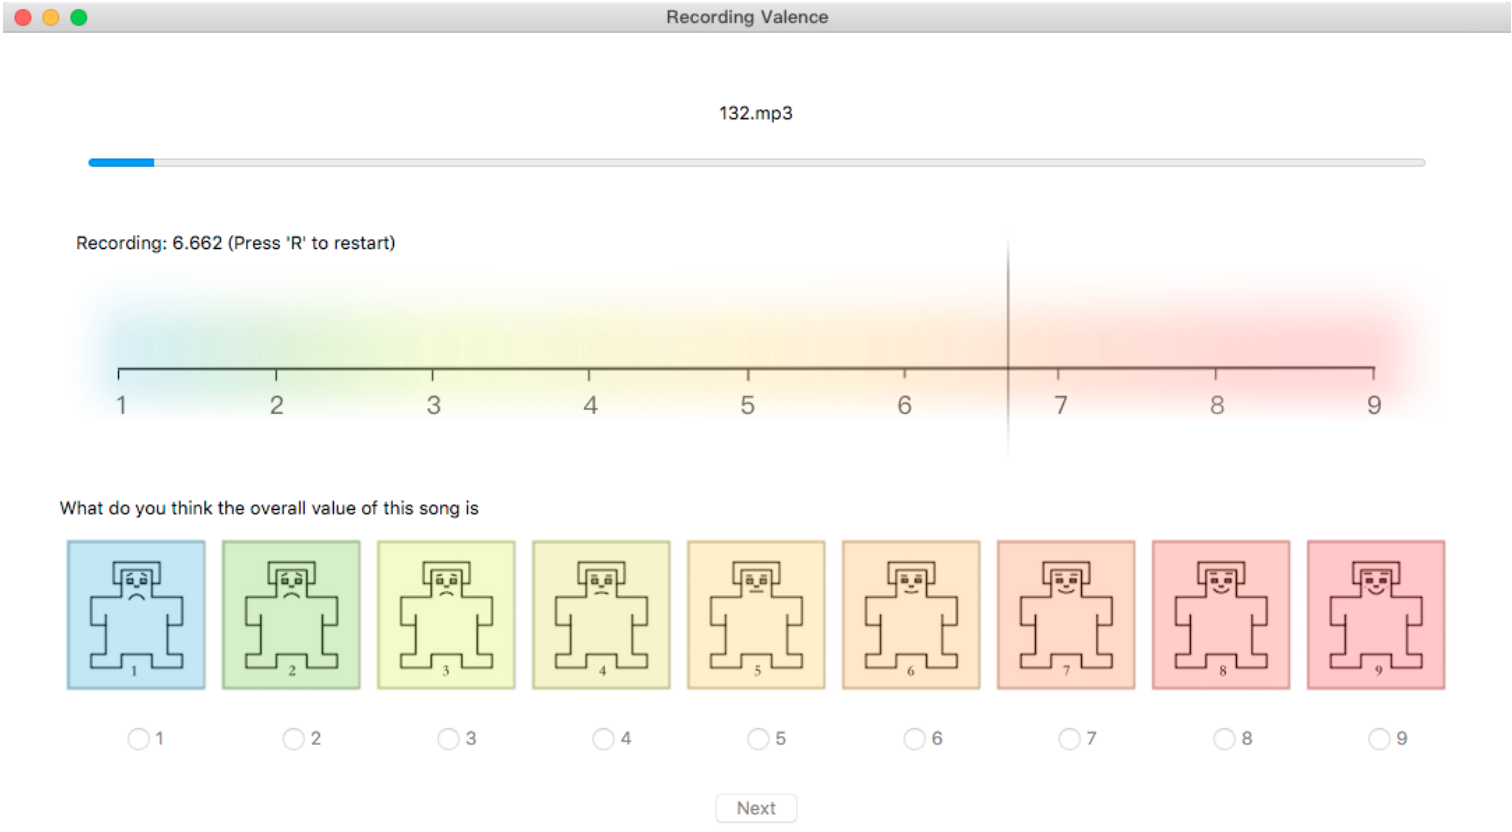
\includegraphics[width=0.65\textwidth]{annotation_interface.png} 
	\caption{Annotation interface for PMEmo}
    \label{fig:annotation_interface}
\end{figure}
\\
In figure \ref{fig:experimental_procedure} is shown the flow diagram of the experiment, where each subject spent $50$ minutes on average.
\begin{figure}[h]
    \centering
    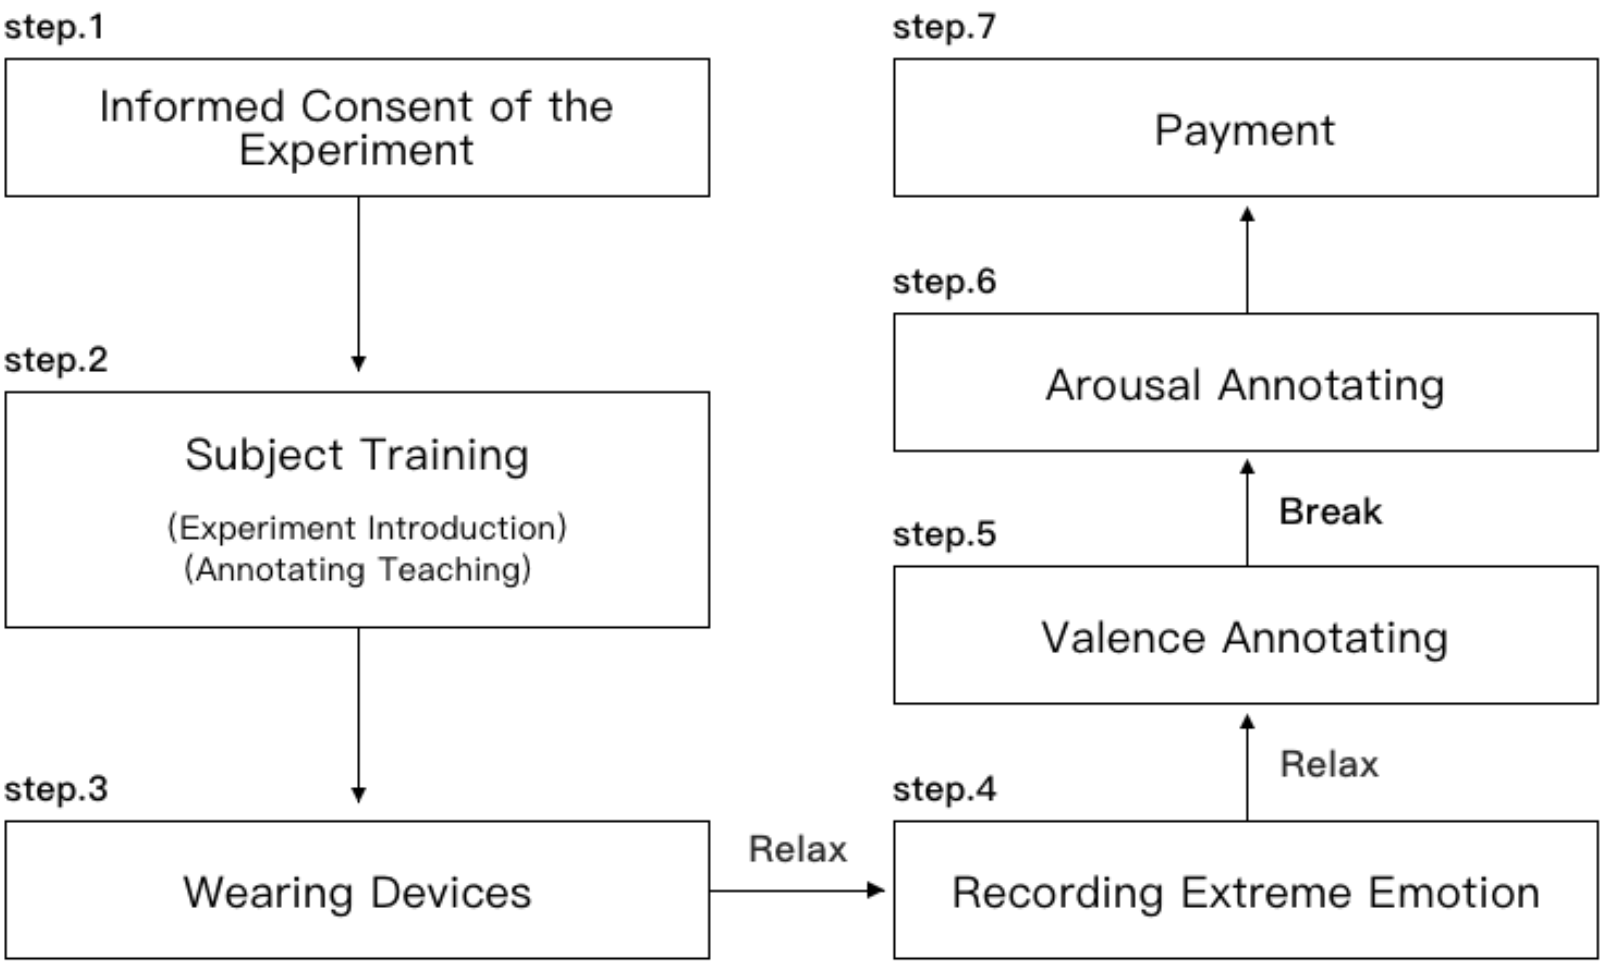
\includegraphics[width=0.7\textwidth]{experimental_procedure.png} 
	\caption{Experimental procedure for PMEmo}
    \label{fig:experimental_procedure}
\end{figure}
\\
Each subject listened to $20$ excerpts and one of those was duplicated to guarantee the high quality data as what was done in \cite{chen2015amg1608}. The annotations from this subjects were accepted only if the bias between duplicate clips were within $0.25$ in the \gls{va} space (they did not inform subjects about the duplicated excerpt).
\\
In total $457$ subjects have participated but $401$ were considered valid annotations ($87.7\%$). Each music clip was annotated by at least $10$ subjects including English speakers and semi-experts from music academy.

\subsection{Data reliability}
As \gls{iot} concept remarks, annotators need some preliminary time before they can give meaningful and reliable annotations. Schubert in \cite{schubert2013reliability} found that median \gls{iot} for valence was $8s$ while for arousal $12s$. Other researchers showed that annotations began to converge after $10s$. The \gls{pmemo} authors decided to discard first $15s$ for the dynamic annotations from the data.
\\ \indent
To evaluate annotation consistency they used the Chronbach's $\alpha$, it represent the degree to which a set of items measures a single unidimensional latent construct. In \cite{zhang2018pmemo} computed the Chronbach's $\alpha$ on the sequence of annotations for each song.
\\
They processed annotations by:
\begin{equation}
	a_{j,i}=a_{j,i}+(\bar{A}_j-\bar{A})
\end{equation}
where:
\begin{itemize}
	\item $a_{j,i}$ is the label annotated by subject $j$ at time $i$
	\item $\bar{A}$ is the mean of all the labels for this song by all subjects
	\item $\bar{A}_j$ is the mean of dynamic labels by subject $j$
\end{itemize}
The mean (averaged across songs) and the standard deviation of the Chronbach's $\alpha$ for the annotation in the \gls{pmemo} dataset are shown in table \ref{table:Chronbach}.
\begin{table}[h!]
	\centering
	\begin{tabular}{|c|c|c|}
		\hline
		Dimension & Mean & Std Dev \\ [0.5ex] 
		\hline\hline Valence & 0.998 & 0.005 \\ 
		\hline Arousal & 0.998 & 0.008 \\ 
		\hline
	\end{tabular}
	\caption{Mean and standard deviation of the Chronbach's $\alpha$ for PMEmo dataset annotations}
	\label{table:Chronbach}
\end{table}

\subsection{Feature set}
As already mentioned before in \ref{music_features}, for generic \gls{mer} there has been no attempt made at defining a "standard" feature set. In PMEmo work \cite{zhang2018pmemo} they based on the INTERSPEECH 2013 \gls{compare} \cite{schuller2013interspeech} and extracted a feature set of 6373-dimension scale.
\\
They provided all $6373$-dimension features in song level for the sake of static emotion task. They extracted only the core of $260$-dimension features in segment level (calculated in $1s$ window with $0.5s$ overlap) for dynamic recognition task to properly reduce the computing load.
\\
Extraction of the features is done with the open-source toolkit \href{https://www.audeering.com/opensmile/}{openSMILE}\footnote{https://www.audeering.com/opensmile/} \cite{eyben2013recent}.
\\
No feature selection procedure was implemented in \gls{pmemo} work.

\subsection{PMEmo performances}
In the article, they adopt \gls{mlr} and \gls{svr} as the base classifiers to model emotions in valence and arousal.
\\
For the static part, they trained and tested the classifiers using all the $6373$-dimension features $x_1,x_2,...,x_{6373}$ and separate static labels of valence $y_{valence}$ and arousal $y_{arousal}$ respectively.
\begin{equation}
	{X_1,X_2,...,X_m} \quad \rightarrow \quad {e_1,e_2,...,e_m}
\end{equation}
where:
\begin{itemize}
	\item $m$ is the number of songs
	\item $X_i={x_1,x_2,...,x_{6373}}$ is the feature set of the $i^{th}$ song
	\item $e_i$ is the value of valence or arousal for this song
\end{itemize}
With respect of continuous mood of a song, is natural to consider a decoupling into two scales and then recognize them separately.
\\
For the dynamic emotion, defined as:
\begin{equation}
	L_i=\bar{L}_i+D_i^{t_i}
\end{equation}
where:
\begin{itemize}
	\item $t_i$ is the number of timestamps in the $i^{th}$ song
	\item $\bar{L}_i$ is the mean of dynamic emotion
	\item $D_i^{t_i}$ is the fluctuation at each timestamp
\end{itemize}
the global model is:
\begin{equation}
	{X_1,X_2,...,X_m} \quad \rightarrow \quad {\bar{L}_1,\bar{L}_2,...,\bar{L}_m}
\end{equation}
while, the local model is:
\begin{equation}
	{Y_1^{t_1},Y_2^{t_2},...,Y_m^{t_m}} \quad \rightarrow \quad {D_1^{t_1},D_2^{t_2},...,D_m^{t_m}}
\end{equation}
where:
\begin{itemize}
	\item $m$ is the number of songs
	\item $X_i$ is the global feature set of it
	\item $Y_i^{t_i}$ is a matrix of 260 columns and $t_i$ rows
\end{itemize}
Before the regression models, they resized all the annotations (both for static and dynamic annotations) into $[0,1]$.
\\ \indent
Static task is to predict the overall emotion of a whole song, represented by a single valence value and arousal value. To train and test, they divided the dataset in $11$ folds, 10 constituted the training set and the remaining set used to test the train model. A 10-fold-cross-validation was used for parameter optimization.
\\
\gls{rmse} and Pearson Correlation Coefficient (r) were calculated separately for valence and arousal. In table \ref{table:PMEmo_results_static} is shown results on static emotions.
\begin{table}[h!]
	\centering
	\begin{tabular}{|c|c|c|c|}
		\hline
		Dimension & Classifier & RMSE & r \\ [0.5ex] 
		\hline\hline Valence & MLR & 0.136 & 0.546 \\ 
		\hline Valence & SVR & 0.124 & 0.638 \\
		\hline Arousal & MLR & 0.111 & 0.719 \\
		\hline Arousal & SVR & 0.102 & 0.764 \\
		\hline
	\end{tabular}
	\caption{Evaluation results on static emotions}
	\label{table:PMEmo_results_static}
\end{table}
\\
About the dynamic case, a hierarchical regression model aiming to recognize the global trend as well as local variation was built. For Global-scale they extracted, for each song, one global feature and mapped it into one global emotion. For Local-scale operation, for each song, they divided it into $1s$ segment with $50\%$ overlap, then extracting the local features from these fragments and project them onto mood space.
\\
In table \ref{table:PMEmo_results_dynamic} is presented the evaluation results on dynamic emotions.
\begin{table}[h!]
	\centering
	\begin{tabular}{|c|c|c|c|c|}
		\hline
		Dimension & Classifier & Scale & RMSE & r \\ [0.5ex] 
		\hline\hline Valence & MLR & global & 0.103 & 0.673 \\
		\hline Valence & MLR & local & 0.016 & 0.047 \\
		\hline Valence & SVR & global & 0.106 & 0.675 \\
		\hline Valence & SVR & local & 0.016 & 0.095 \\
		\hline Arousal & MLR & global & 0.113 & 0.816 \\
		\hline Arousal & MLR & local & 0.020 & 0.103 \\
		\hline Arousal & SVR & global & 0.101 & 0.844 \\
		\hline Arousal & SVR & local & 0.019 & 0.115 \\
		\hline
	\end{tabular}
	\caption{Evaluation results on dynamic emotions}
	\label{table:PMEmo_results_dynamic}
\end{table}
\\
In \gls{pmemo} work, as already mentioned, they also recorded \gls{eda} subjects data when they were listening to music.
\\
On \gls{eda}, they employed a low-pass filter of $0.6Hz$ to diminish the noise due to motion artifacts. Then skin electric conductance was scaled in z-score:
\begin{equation}
	z-score=\dfrac{X-\mu}{\sigma}
\end{equation}
where $\mu$ is the mean of vector $X$ and $\sigma$ is the standard variation.
Last passage on \gls{eda} signal was to resample them, from $50Hz$ to $2Hz$ due to different acquisition of EDA and continuous emotions.
\\
They trained and tested \gls{mlr} and \gls{svr} with pre-processed \gls{eda} data in the dynamic case and results are shown in table \ref{table:PMEmo_results_EDA}.
\begin{table}[h!]
	\centering
	\begin{tabular}{|c|c|c|c|c|}
		\hline
		Dimension & Classifier & Scale & RMSE & r \\ [0.5ex] 
		\hline\hline Valence & MLR & global & 0.139 & 0.063 \\
		\hline Valence & MLR & local & 0.016 & 0.060 \\
		\hline Valence & SVR & global & 0.141 & 0.017 \\
		\hline Valence & SVR & local & 0.016 & 0.059 \\
		\hline Arousal & MLR & global & 0.186 & 0.011 \\
		\hline Arousal & MLR & local & 0.019 & 0.097 \\
		\hline Arousal & SVR & global & 0.194 & 0.040 \\
		\hline Arousal & SVR & local & 0.019 & 0.099 \\
		\hline
	\end{tabular}
	\caption{Evaluation results on dynamic EDA}
	\label{table:PMEmo_results_EDA}
\end{table}

\section{Implementation}
We decided to start from the results of \gls{pmemo} and try to improve them. We will first look at a general framework description and then will follow explanation of the single parts.

\subsection{General framework}
As already presented in chapter \ref{general_methodology} in figure \ref{fig:emotion_recognition_process} through some steps we can derive a model from the emotion elicitation. Since we will try to deal with both audio and \gls{eda} data, we decided to develop a model based on a traditional machine learning framework.
\\
General framework implemented is in figure \ref{fig:general_framework}. Differently from figure \ref{fig:emotion_recognition_process}, here, the starting point is dataset files given from the \gls{pmemo} dataset.
\begin{figure}[h]
    \centering
    \includegraphics[width=\textwidth]{general_framework.png} 
	\caption{General framework}
    \label{fig:general_framework}
\end{figure}
\\
From the dataset containing audio and \gls{eda} files, we extracted a certain number of features, creating a matrix for all the features extracted.
\\
From the feature matrix, several feature selection algorithms were applied in order to reduce the number of features, to improve the model.
\\
At last, some \gls{ml} process is applied to create the model for the emotion classification task and then it is tested.
\\
In this dataset were present two different types of data, audio and \gls{eda} and our main goal was to combine:
\begin{itemize}
	\item audio data,which gave the possibility to recognize perceived emotions
	\item \gls{eda} data, which are related to felt emotions
\end{itemize}
The general framework, with these two process divided is shown in figure \ref{fig:general_framework_1} which is based on the one presented before at \ref{fig:general_framework}.
\begin{figure}[h]
    \centering
    \includegraphics[width=\textwidth]{general_framework_1.png} 
	\caption{General framework with audio and EDA division}
    \label{fig:general_framework_1}
\end{figure}
\\[5px]
Now will be presented the first part of the general framework, feature extraction block, separated for audio and for \gls{eda}, due to evident differences in data types. For the audio, there are several set of features that can be extracted, thanks to the hard work done in the past years. While \gls{eda} features are less present in the literature and they are mostly statistical features.

\subsection{Audio features}
For the next features explanation, will be used the song contained in the \gls{pmemo} dataset under the name \textit{4.mp3}, \textit{X Bitch} from \textit{21 Savage} in the album "\textit{Savage mode}". Its waveform and audio specs can be seen in figure \ref{fig:audio_specs}.
\begin{figure}[h]
    \centering
    \includegraphics[width=\textwidth]{audio_specs.png} 
	\caption{Waveform and audio specs of the song number 4}
    \label{fig:audio_specs}
\end{figure}
\\
Now will follow a list of features extracted during the process.
\\
Features was extracted both in a static way, taking into account the whole excerpt and in a dynamic way, by dividing the musical excerpt in windows of $1s$ with $50\%$ overlap.
\\
After the process of feature extraction, every feature was normalized in the range $[0,1]$.
\paragraph{Tempo}
\mbox{} \\ \\
In musical terminology, tempo  is the speed or pace of a given piece. In classical music, tempo is typically indicated with an instruction at the start of a piece and is usually measured in beats per minute (or bpm).
\\
Tempo for the given song is about $152 bpm$.

\paragraph{Beats}
\mbox{} \\ \\
To extract beats is used a beat extractor, which output is an estimation of the tempo and an array of frame numbers corresponding to detected beat events.
\\
Beats are detected in three stages:
\begin{enumerate}	
	\item Measure onset strength
	\item Estimate tempo from onset correlation
	\item Pick peaks in onset strength approximately consistent with estimated tempo
\end{enumerate}
In figure \ref{fig:beat} can be seen beats detected and the array of frame numbers.
\begin{figure}[h]
    \centering
    \includegraphics[width=\textwidth]{beat.png} 
	\caption{Beat and array of frames of the song number 4}
    \label{fig:beat}
\end{figure}
\\
After the beats extraction, summation and average of the beat events are calculated.

\paragraph{Zero crossing rate}
\mbox{} \\ \\
The \gls{zcr}  is the rate of sign-changes along a signal. It is the rate at which the signal changes from positive to zero to negative or to negative or from negative to zero to positive. It is useful to recognize percussive sounds.
The \gls{zcr} is evaluated as:
\begin{equation}
	ZCR=\dfrac{1}{T} \sum_{t=1}^{T-1}{\dfrac{|sign(s_t)|-|sign(s_{t-1})|}{2}}
\end{equation}
where $T$ is the length of the time window, $s_t$ is the magnitude of the $t^{th}$ time domain sample.
\\
The \gls{zcr} of song 4 is shown in figure \ref{fig:zcr}.
\begin{figure}[h]
    \centering
    \includegraphics[width=\textwidth]{zcr.png} 
	\caption{ZCR extracted from song 4}
    \label{fig:zcr}
\end{figure}
\\
For the \gls{zcr}, is calculated the mean, the standard deviation, and the variance.

\paragraph{Chroma}
\mbox{} \\ \\
The chroma feature, also called chromagram, relates to the twelve different pitch classes. Chroma features capture harmonic and melodic characteristic of music, while being robust to changes in timbre and instrumentation.
\\
Humans perceive two musical pitches as similar if they differ by an octave. A pitch can be separated into two components, referred as \textit{height} (the octave where the pitch is) and \textit{chroma}. The twelve chroma values are represented by the set:
\[{C, C\#, D, D\#, E , F, F\#, G, G\#, A, A\#, B}\]
that consists of the twelve pitch spelling attributes as used in Western music notation.
\\
In the figure \ref{fig:chromagram} from \cite{inproceedings} can be seen a chromagram (b) obtained from the score (a) and a chromagram (d) obtained from an audio recording of the C-major scale played on a piano (c).
\begin{figure}[h]
    \centering
    \includegraphics[width=0.8\textwidth]{chromagram.png} 
	\caption{(a) Musical score of a C-major scale, (b) Chromagram obtained from the score, (c) audio recording of the C-major scale played on a piano, (d) chromagram obtained from the audio recording from \cite{inproceedings}}
    \label{fig:chromagram}
\end{figure}
\\
There are different ways to convert an audio recording into a chromagram, as performing \gls{stft} in combination with binning strategies or using multirate filter banks.
\\ \indent
Chroma features can be significantly changed by introducing pre-processing and post-processing steps that modify spectral, temporal and dynamical aspects. This leads to a large number of chroma variants.
\\
For the chromagram, we extracted three different types of chroma:
\begin{itemize}
	\item Chroma \gls{stft} extract the chromagram through the \gls{stft}.
	\item Chroma cqt extract the constant-Q chromagram, where the constant-Q transforms the data series to the frequency domain. Q stands for the quality factor, defined as:
	\begin{equation}
		Q=\dfrac{f_k}{\delta f_k}
	\end{equation}
	where $f_k$ is the $k^{th}$ filter while $\delta f_k$ is the bandwidth of the $k^{th}$ filter.
	\item Chroma cens which consider short-time statistics over energy distribution within the chroma bands. In \gls{cens} features, a quantization is applied based on logarithmic thresholds, which introduce a temporal smoothing.
\end{itemize}
In the figure \ref{fig:chroma} are shown the three different chromagram extracted for the song number 4.
\begin{figure}[h]
    \centering
    \begin{subfigure}{{\textwidth}}
    		\includegraphics[width=\textwidth]{chroma_stft.png}
    		\caption{Chroma stft}
    \end{subfigure}
    \begin{subfigure}{\textwidth}
    		\includegraphics[width=\textwidth]{chroma_cqt.png} 
    		\caption{Chroma cqt}
    \end{subfigure}
    \begin{subfigure}{\textwidth}
    		\includegraphics[width=\textwidth]{chroma_cens.png} 
    		\caption{Chroma cens}
    \end{subfigure}
    \caption{Different chromagram extracted from song number 4}
    \label{fig:chroma}
\end{figure}
\\
For every type of chromagram, is calculated the mean, the standard deviation, and the variance.

\paragraph{Melspectrogram}
\mbox{} \\ \\
The melspectrogram is a mel-scaled spectrogram. A spectrogram is a visual representation of the spectrum of frequencies of a signal as it varies with time. It can be generated by a bank of band-pass filter, by Fourier transform or \gls{dwt}.
\\ \indent
In order to have a more comprehensible spectrogram, when dealing with audio signals, it is scaled. The axis representing the frequencies is transformed to log scale, and the \textit{color} axis representing the amplitude, is scaled to Decibels, kinda of the log scale of amplitudes.
\\ \indent
The Mel-scale is a different scale, based on non-linear transformation of the frequency scale. It is constructed such that sounds of equal distance from each other on the Mel-scale also \textit{sound} to humans as they are equal in distance from one another.
\\
In practice it partitions the $Hz$ scale into bins, and transforms each bin into a corresponding bin in the Mel Scale, using a overlapping triangular filters.
\\
To convert a frequency in $Hz$ into its equivalent in $mel$, the following formula is used:
\begin{equation}
	pitch[mel]=1127.0148\:\log \left[ {1+\dfrac{f}{100}} \right]
\end{equation}
\\
Finally, a melspectrogram is a spectrogram with the mel-scale on the frequency axis.
\\
The melspectrogram of song 4 is shown in figure \ref{fig:melspectrogram}.
\begin{figure}[h]
    \centering
    \includegraphics[width=\textwidth]{melspectrogram.png} 
	\caption{Melspectrogram extracted from song 4}
    \label{fig:melspectrogram}
\end{figure}
\\
For the melspectrogram, is calculated the mean, the standard deviation, and the variance.

\paragraph{Spectral contrast}
\mbox{} \\ \\
Spectral contrast consider spectral peaks and valleys in each sub-band separately. More in general spectral peaks correspond to harmonic components and spectral valleys correspond to non-harmonic components or noise in a music piece as evaluated in \cite{jiang2002music}.
\\
Therefore, the difference between spectral peaks and spectral valleys will reflect the spectral contrast distribution.
\\
The spectral contrast of song 4 is shown in figure \ref{fig:spectral_contrast}.
\begin{figure}[h]
    \centering
    \includegraphics[width=\textwidth]{spectral_contrast.png} 
	\caption{Spectral contrast extracted from song 4}
    \label{fig:spectral_contrast}
\end{figure}
\\
For the spectral contrast, is calculated the mean, the standard deviation, and the variance.

\paragraph{Spectral centroid}
\mbox{} \\ \\
Spectral centroid is a measure to characterize a spectrum. It indicates where is located the center of mass of the spectrum. It has connection with the brightness of a sound.
\\
Spectral centroid is calculated as a weighted mean of the frequencies present in the signal, determined using a Fourier transform, with their magnitudes as the weights:
\begin{equation}
	cent=\dfrac{\sum_{n=0}^{N-1}{f(n)x(n)}}{\sum_{n=0}^{N-1}{x(n)}}
\end{equation}
where $x(n)$ is the weighted frequency value (or magnitude) of bin number $n$ and $f(n)$ represents the center frequency of that bin.
\\
The spectral centroid of song 4 is shown in figure \ref{fig:spectral_centroid}.
\begin{figure}[h]
    \centering
    \includegraphics[width=\textwidth]{spectral_centroid.png} 
	\caption{Spectral centroid extracted from song 4}
    \label{fig:spectral_centroid}
\end{figure}
\\
For the spectral centroid, is calculated the mean, the standard deviation, and the variance.

\paragraph{Spectral bandwidth}
\mbox{} \\ \\
The spectral bandwidth is the order-p spectral bandwidth as:
\begin{equation}
	{\left(\sum_{k}{S(k){(f(k)-f_c)}^p}\right)}^{1/p}
\end{equation}
where $S(k)$ is the spectral magnitude at frequency bin $k$, $f(k)$ is the frequency at bin $k$ and $f_c$ is the spectral centroid.
\\
The spectral bandwidth of song 4 is shown in figure \ref{fig:spectral_bandwidth}.
\begin{figure}[h]
    \centering
    \includegraphics[width=\textwidth]{spectral_bandwidth.png} 
	\caption{Spectral bandwidth extracted from song 4}
    \label{fig:spectral_bandwidth}
\end{figure}
\\
For the spectral bandwidth, is calculated the mean, the standard deviation, and the variance.

\paragraph{Spectral rolloff}
\mbox{} \\ \\
Spectral rolloff is defined as the $N^{th}$ percentile of the power spectral distribution, where $N$ is usually $85 \%$ or $95 \%$. The rolloff point is the frequency below which the N of the magnitude distribution is concentrated.
\\
This can be used to, e.g., approximate the maximum (or minimum) frequency by setting roll\_percent to a value close to $1$ (or $0$).
\\
The spectral rolloff of song 4 is shown in figure \ref{fig:spectral_rolloff}.
\begin{figure}[h]
    \centering
    \includegraphics[width=\textwidth]{spectral_rolloff.png} 
	\caption{Spectral rolloff extracted from song 4}
    \label{fig:spectral_rolloff}
\end{figure}
\\
For the spectral rolloff, is calculated the mean, the standard deviation, and the variance.

\paragraph{Spectral poly}
\mbox{} \\ \\
Get coefficients of fitting an $n^{th}$ order polynomial to the columns of a spectrogram.
\\
In the figure \ref{fig:poly} can be seen different poly extracted from song number 4, with different degrees, 0-order fit a degree-0 polynomial (constant) to each frame, 1-order fit a linear polynomial to each frame and 2-order fit a quadratic to each frame.
\begin{figure}[h]
    \centering
    \includegraphics[width=\textwidth]{poly.png} 
	\caption{Spectral poly extracted from song 4}
    \label{fig:poly}
\end{figure}
\\
For the spectral poly, is calculated the mean, the standard deviation, and the variance.

\paragraph{Tonal centroid}
\mbox{} \\ \\
Computes the tonal centroid features (tonnetz), following the method of \cite{harte2006detecting}.
\\
In musical tuning and harmony, the Tonnetz, is a conceptual lattice diagram representing tonal space first described by Euler in 1739. Various visual representations of the Tonnetz can be used to show traditional harmonic relationships in European classical music.
\\
Close harmonic relations are modeled as short distances on an infinite Euclidian plane. Chords become geometric structure on the plane and chords become geometric structures on the plane, keys are defined by regions in the harmonic network
\\
An example is shown in figure \ref{fig:tonnetz_scheme}.
\begin{figure}[h]
    \centering
    \includegraphics[width=\textwidth]{tonnetz_scheme.png} 
	\caption{Representation in the Euclidian plane of the tonnetz}
    \label{fig:tonnetz_scheme}
\end{figure}
\\
The Tonnetz of the song number 4 is shown in figure \ref{fig:tonnetz}.
\\
\begin{figure}[h]
    \centering
    \includegraphics[width=\textwidth]{tonnetz.png} 
	\caption{Tonnetz extracted in from song 4}
    \label{fig:tonnetz}
\end{figure}

\paragraph{Mel Frequency Cepstral Coefficients}
\mbox{} \\ \\
The \gls{mfcc} are coefficients based on the extraction of the signal energy within critical frequency bands by means of a series of triangular filters (in figure \ref{fig:mfcc_filters}) whose center frequencies are equally spaced according to the mel scale.
\begin{figure}[h]
    \centering
    \includegraphics[width=0.6\textwidth]{mfcc_filters.png} 
	\caption{Triangular filters for the MFCC extraction}
    \label{fig:mfcc_filters}
\end{figure}
\\
The log-energy of the spectrum is measured within the pass-band of each filter, resulting in a reduced representation of the spectrum. The cepstral coefficients are finally obtained through a \gls{dct} of the reduced log-energy spectrum.
\\
In figure \ref{fig:mfcc} is shown the \gls{mfcc} graph for 12 mfccs for song number 4.
\begin{figure}[h]
    \centering
    \includegraphics[width=\textwidth]{mfcc.png} 
	\caption{MFCC for song 4}
    \label{fig:mfcc}
\end{figure}
\\
For each of the 12 mfccs are extracted the mean, standard deviation, median, kurtosis and skewness.

\subsection{EDA features}
For the continuity, also in the explanation of \gls{eda} features extracted, will be used the song number 4. Its \gls{eda} signal and its specs, can be seen in figure \ref{fig:eda}.
\begin{figure}[h]
    \centering
    \includegraphics[width=\textwidth]{eda.png} 
	\caption{EDA for song 4}
    \label{fig:eda}
\end{figure}
\\
\gls{eda} signal was preprocessed following the pipeline highlighted in the pyphysio library \cite{bizzego2019pyphysio} and resumed in figure \ref{fig:pyphysio_pipeline}.
\begin{figure}[h]
    \centering
    \includegraphics[width=\textwidth]{pyphysio_pipeline.png} 
	\caption{Pyphysio pipeline}
    \label{fig:pyphysio_pipeline}
\end{figure}
\\
They divide the pipelines into three separate steps:
\begin{enumerate}
	\item Filtering and Preprocessing: this step includes all the procedures aiming at increasing the signal/noise ratio, typycally band-pass filtering, smoothing, removal of artifacts. The output of this step is a new version of the imput signal with improved signal quality (less noise)
	\item Information Extraction: this step aims at extracting the information of interest from the physiological signal. The output is a new signal containing only the information of interest and thus it has a signal\_nature different from the input signal
	\item Physiological Indicators: this steps produces a list of scalar values able to describe the characteristics of the input signal. This step is usually performed on small segments of the input signals which are extracted using a sliding window on the whole length of the signal.
\end{enumerate}
Taking into account the initial signal shown in figure \ref{fig:eda} the filtering and preprocessing stage was done by an \gls{iir} filter to remove high frequency noise, a low-pass filter of $0.6Hz$ to diminuish the noise from motion and artifacts as can be seen in figure \ref{fig:eda_filtered}.
\begin{figure}[h]
    \centering
    \includegraphics[width=\textwidth]{eda_filtered.png} 
	\caption{EDA signal in blue and filtered EDA in orange}
    \label{fig:eda_filtered}
\end{figure}
\\
Following the procedure introduced by \cite{bizzego2019pyphysio}, the library is able to extract tonic and phasic component of an \gls{eda} data by evaluating a driver function. The graph can be seen in figure \ref{fig:eda_phasic_driver}.
\begin{figure}[h]
    \centering
    \includegraphics[width=\textwidth]{eda_phasic_driver.png} 
	\caption{EDA signal in blue, driver in orange and tonic part in green}
    \label{fig:eda_phasic_driver}
\end{figure}
\\
Now will follow a list of features extracted during the process.
\\
Features was extracted both in a static way, taking into account the whole excerpt and in a dynamic way, by dividing the musical excerpt in windows of $1s$ with $50\%$ overlap.
\\
After the process of feature extraction, every feature was normalized in the range $[0,1]$.

\paragraph{Statistic}
\mbox{} \\ \\
As already mentioned before in \ref{EDA_features}, most extracted \gls{eda} features are statistical. We extracted the mean of the signal, the standard deviation, kurtosis and the skewness. They were extracted both in the time domain and in the frequency domain.
\\ \indent
Median value was also extracted, where the median is the value separating the higher half from the lower half of the data. It is like the \textit{middle} value, but differently from the mean, the median gives a better idea of a typical value.
\\
While other statistics were already described in \ref{EDA_features}, the median can be described in a caseless formula as:
\begin{equation}
	median(a)=\dfrac{a_{\left \lceil{\dfrac{l+1}{2}}\right \rceil}+a_{\left \lfloor{\dfrac{l+1}{2}}\right \rfloor}}{2}
\end{equation}
where $a$ is an ordered list of $l$ numbers, $\left \lceil {\cdot} \right \rceil$ is the ceil function (gives the least integer greater than or equal to the input) and $\left \lfloor {\cdot} \right \rfloor$ is the floor function (gives the greatest integer less than or equal to the input).
\\ \indent
We extracted also the maximum value, the minimum and the difference between these two, the range.

\paragraph{Other features}
\mbox{} \\ \\
Some other features were extracted thanks to pyphisio library \cite{bizzego2019pyphysio}, they are:
\begin{itemize}
	\item \gls{auc}
	\item \gls{rmssd} compute the \gls{rmse} of the squared $1^{st}$ order discrete differences
	\item \gls{sdsd} calculate the standard deviation of the $1^{st}$ order discrete differences
\end{itemize}

\paragraph{Power inband}
\mbox{} \\ \\
The power spectrum $S_{xx}(f)$ of a time series $x(t)$ describes the distribution of power into frequency components compsing the signal. Any discrete signal, according to Fourier analysis, can be decomposed into a number of discrete frequencies, or a spectrum of frequencies over a continuous range.
\\
The statistical average of a certain signal as analyzed in terms of its frequency content, is called its spectrum.
\\ \indent
The \gls{psd}, also called power spectrum, applies to signal over all time, that theoretically could be an infinite time interval. The \gls{psd} than, refers to the spectral energy distribution that would be found per unit time, since the total energy of such a signal over all time would generally be infinite.




\paragraph{Peak inband}
\mbox{} \\ \\ 
	\chapter{Results and Improvements}
\label{chap:Improvements}
\pagestyle{plain}
\vspace{0.5cm}

\noindent In this chapter we present...

Then...

Finally ...


\section{Some different sections}

\section{Conclusive Remarks}
 
	\chapter{Conclusions and Future Works}
\label{chap:Conclusions}
\thispagestyle{plain}
\vspace{0.5cm}

\noindent

This work of thesis proposes a methodology for...

The devised methodology is based on...

The main advantages are...

As far as the experiments are concerned...

The proposed approach has shown promising results both in simulation and in the experiments.


\section{Future Works}

\paragraph{Generalization}
We would like to generalize...

\paragraph{Challenging scenarios}
Another possible improvement is related to the extension of the proposed approach to...

\paragraph{Different approaches}
Finally we are moving towards a deeper analysis of...
a
a
a
a
a
a
a
a
a
a
a
a
a
a
a
 	
	\appendix
\chapter*{Appendices}
\addcontentsline{toc}{chapter}{Appendices} % note that the appendices names can differ from the "chapter" title in the toc.
\renewcommand{\thesection}{\Alph{section}} % sections are not listed with numbers but with letters.
 
\thispagestyle{plain}

\section{Equipment 1}
\label{appendix:equipment}

\section{Proofs of Mathematical Theories1}
\label{appendix:math} 
	
	%% print the bibliography
	%\nocite{*}
	\bibliographystyle{ieeetr} % IEEE has its own bibliography style. Bibtex is the baseline bibliography engine, you can use also biber to gain control on the layout.
	\bibliography{../bibliography}

\end{document}